\documentclass[mscthesis]{usiinfthesis}
\usepackage{lipsum}
\usepackage{float}
\usepackage{listings}
\usepackage{wrapfig}

\lstdefinelanguage{algebra}
{morekeywords={import,sort,constructors,observers,transformers,axioms,if,
else,end},
sensitive=false,
morecomment=[l]{//s},
}



\title{Sensorial software evolution comprehension} %compulsory
\specialization{Dependable Distributed Systems}%optional
\subtitle{Subtitle: Reinventing the World} %optional 
\author{Gianlorenzo Occhipinti} %compulsory
\begin{committee}
\advisor{Prof.}{Michele}{Lanza} %compulsory
\coadvisor{Prof.}{Csaba}{Nagy}{} %optional
\coadvisor{Prof.}{Csaba}{Nagy}{} %optional
\end{committee}
\Day{Yesterday} %compulsory
\Month{July} %compulsory
\Year{2022} %compulsory, put only the year
\place{Lugano} %compulsoyr

\dedication{To my beloved} %optional
\openepigraph{Someone said \dots}{Someone} %optional

%\makeindex %optional, also comment out \theindex at the end

\begin{document}

\maketitle %generates the titlepage, this is FIXED

\frontmatter %generates the frontmatter, this is FIXED

\begin{abstract}
The comprehension of software evolution is essential for the understandability and maintainability of systems.
However, the sheer quantity and complexity of the information generated during systems development make the comprehension process challenging.
We present an approach, based on the concept of synesthesia (the production of a sense impression relating to one sense by stimulation of another sense), which represents the evolutionary process through an interactive visual depiction of the evolving software artifacts complemented by an auditive portrayal of the evolution.
The approach is exemplified in SYN, a web application, which enables sensorial software evolution comprehension.
We applied SYN on real-life systems and presented several insights and reflections. 
\end{abstract}


\begin{acknowledgements}
ACK
\end{acknowledgements}

\setcitestyle{numbers}


\tableofcontents 
\listoffigures %optional
\listoftables %optional

\mainmatter

\chapter{Introduction}

In 1971 Dijkstra made an analogy between computer programming and art \cite{Dijkstra1971a}.
It stated that it is not essential to learn how to compose software but instead, it is necessary to develop its own style and implications. 
During the lifetime of a software system, many developers work on it, each one in their manner. This is one of the multiple reasons behind software complexity. 
Today's systems are characterized by sheer size and complexity. Software maintenance takes up the most of a system's cost. 
It is hard to quantify the impact of software maintenance on the global cost of the software. 
However, Researchers estimated it to be between 50\% and 90\% \cite{Davis1995} \cite{Sommerville1995}\cite{Erlikh2000} \cite{seacord2003}.
Many factors influence the cost of maintenance; among these, there is the understanding activity needed to perform maintenance tasks \cite{Corbi1989}. 

The comprehension of software evolution is essential for the understandability and, consequently, maintainability of systems.
However, the sheer quantity and complexity of the information generated during systems development challenge the comprehension process.

Lehman and Belady, in 1985, were the first to observe that maintaining a software system becomes a more complex activity over time. \cite{Lehman1985}
The term "software evolution" was used for the first time in their set of laws. 
One of the goals of its analysis is to identify potential defects in the system's logic or architecture. 
Visualization techniques often support software evolution analysis.
\bigbreak
Software visualization is a specialization of information visualization with a focus on software \cite{Lanza2003}. In literature, a lot of visualization techniques have been presented to support 
a complex software system's analysis.
Usually, a massive quantity of multivariate evolutionary data needs to be depicted. Several tools have been proposed in the literature to do that \cite{Merino2018a}.

Moreover, numerous techniques have been presented in the literature to facilitate program comprehension. 
The main challenge that each visualization technique has to deal with, is to identify the relevant aspects to be depicted and effectively present them. 
The effectiveness of a software visualization technique could be enhanced by combining it with audio. 
The term "program auralization" was coined for this reason, and it aims to communicate information about the program in an auditory way.
Several studies were done to measure the advantages given by audio as a communication medium \cite{Alty1995}. 


In this work, our focus is an explorative visualization that depicts the evolution of a system.
We present an approach with an evolutionary design-level visualization to facilitate the comprehension of the system's history. 
Our technique models and mines efficiently large git repositories. We also offer a visualization strategy based on the concept of synesthesia 
(the production of a sense impression relating to one sense by stimulation of another sense), 
which represents the evolutionary process through an interactive visual depiction of the evolving software artifacts complemented by an auditive portrayal of the evolution. 

\section{Contribution}
We can summarize the main contribution of this work as follows:
\begin{itemize}
 \item We proposed an approach to model the history of a large git repository.
 \item We proposed an approach to mine large git repositories.
 \item We proposed an approach based on synesthesia, which represents the evolutionary process through an interactive visual depiction of the evolving software artifacts complemented by an auditive portrayal of the evolution.
 \item We engineered a tool, SYN, which supports our approach as an interactive web application
 \item We applied SYN to real-life systems and presented several insights and reflections. 
\end{itemize}

\section{Structure of the document}
This document is organized as follows
\begin{itemize}
 \item {Chapter 1}
 \item {Chapter 2}
 \item {Chapter 3}
 \item {Chapter 4}
 \item {Chapter 5}

\end{itemize}


\chapter[Related Works]{State of the art}
\graphicspath{ {images/stateOfArt} }



\section{Software visualization}


\begin{wrapfigure}{r}{0.3\textwidth}

  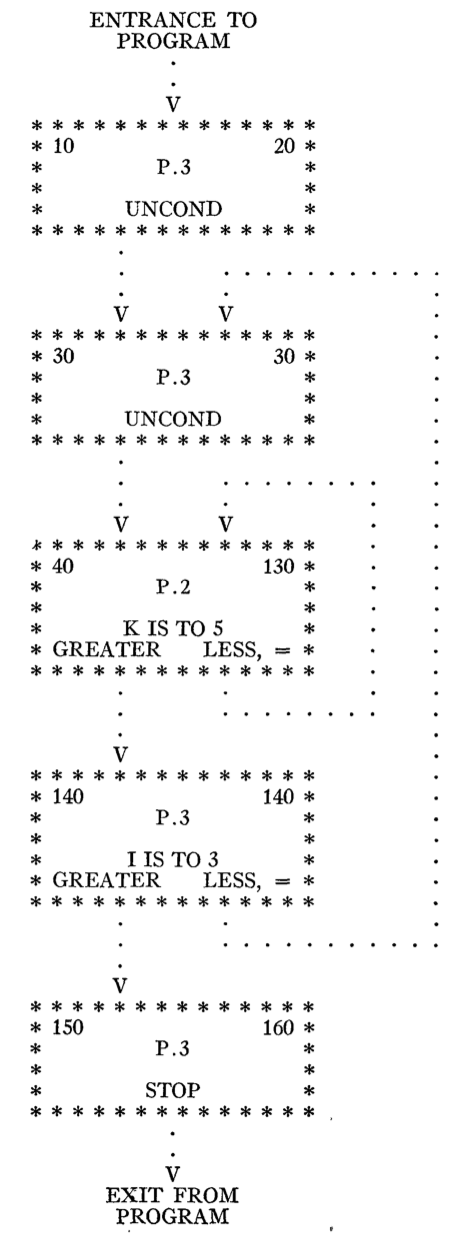
\includegraphics[width=0.9\linewidth]{Haibt1959_Flowchart.png} 
  \caption{Flowchart presented by Haibt in 1959}
  \label{fig:Haibt1959_Flowchart}

\end{wrapfigure}

Software maintenance and evolution are essential parts of the software development lifecycle. Both require that developers deeply understand their system. 
Mayrhauser and Vans defined {\it program comprehension} as a process that "{\it knowledge to acquire new knowledge}" \cite{VonMayrhauser1995}. 
Generally, programmers possess two types of knowledge: general knowledge and software-specific knowledge. 
Software comprehension aims to increase this specific knowledge of the system, and, it can leverage some software visualization techniques for this purpose. 
Software visualization supports the understanding of software systems
by visually presenting various information about them, e.g., their architecture, source code, or behavior.
Stasko et al.\cite{Stasko2008} conducted a study in 1998 that shows how visualization arguments human memory since 
it works as external cognitive aid and thus, improves thinking and analysis capabilities.

% \subsection*{History of software visualization}


\bigbreak

The earliest software visualization techniques in the literature used 2D diagrams. 
For example, Haibt, the first to use them in 1959, provided a graphical outline of a program and its behavior with flowcharts \cite{Haibt1959}. 
As shown in Figure \ref{fig:Haibt1959_Flowchart}, they were 2D diagrams that described the execution of a program.
He wrapped each statement in a box, representing the control flow with arrows.

 \bigbreak
Ten years later, Knuth also confirmed the effectiveness of flowcharts \cite{Knuth1963}. 
He evidenced that programs, around that time, were affected by a lack of readability.
Therefore, he introduced a tool to generate visualizations from the software documentation automatically.

\bigbreak
Nassi and Schneiderman\cite{Nassi1973}, in 1973, introduced the Nassi–Shneiderman diagram (NSD), able to represent the structure of a program. 
The diagram was divided into multiple sub-block, each with a given semantic based on its shape and position. 

\bigbreak
The 80s registered two main directions of software visualization. The first was the source code presentation.
For example, Hueras and Ledgard \cite{Hueras1977} then Waters \cite{Waters1983} developed techniques to format the source code with a prettyprinter. 
The second direction was the program behavior, used mainly for educational purposes. One of that period's most prominent visualization systems was Balsa-II \cite{Brown1988}.
 
\bigbreak
Balsa-II was a visualization system that, through animations, displayed the execution of an algorithm.
Programmers were able to customize the view and the control execution of the algorithm, to understand them with a modest amount of effort. 
The program was domain-independent, and users could use it with any algorithm. 

\bigbreak
Around the end of the 80s, Müller et al. \cite{Mueller1988} released Rigi, a tool used to visualize large programs.
It exploited the graph model, augmented with abstraction mechanisms, to represent systems components and relationships. 

\begin{figure}[H]
  \minipage{0.33\textwidth}
    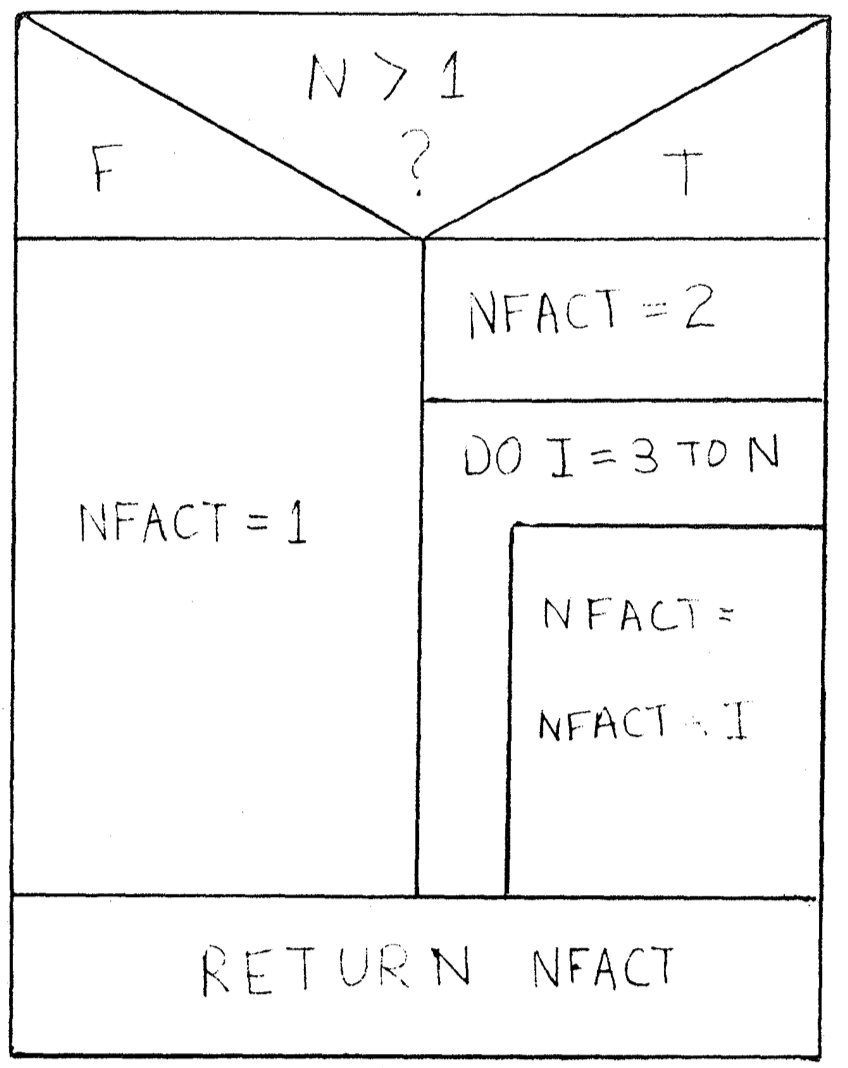
\includegraphics[width=0.8\linewidth]{Nassi1973_NSD.png}
    \label{fig:Nassi1973_NSD}
    \caption{NSD of the factorial function.}
  \endminipage\hfill
  \minipage{0.33\textwidth}
    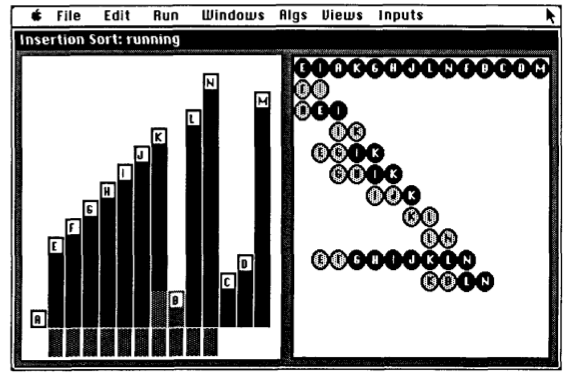
\includegraphics[width=\linewidth]{Brown1988_BalsaII.png}
    \caption{Balsa-II}
  \endminipage\hfill
  \minipage{0.33\textwidth}
  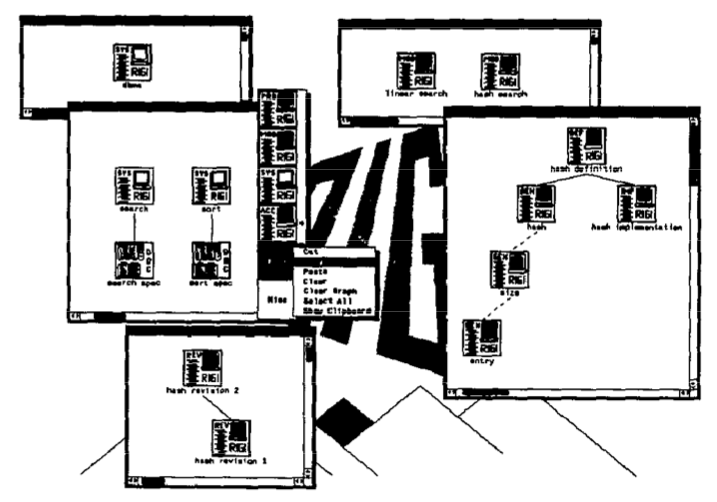
\includegraphics[width=\linewidth]{Mueller1988_Rigi.png}
  \caption{Rigi}
\endminipage\hfill
  \end{figure}


  % The growing number of object-oriented programming languages emerging in the mainstream raised 
  % the interest in understanding not only the structure but also the behavior of systems written according to this paradigm. 
  % Kleyn et al. proposed GraphTrace [KG88], a tool using concurrently animated views to visualize dynamic information,
  % Myers's taxonomy of program visualization systems
  % Price et al. proposed a more detailed taxonomy

\bigbreak
The 1990s recorded more interest in the field of software visualization. 
In 1992, Erik et al. introduced a new technique to visualize line-oriented statistics \cite{Eick1992}. 
It was embodied in Seesoft, a software visualization system to analyze and visualize up to 50,000 lines of code simultaneously. 
On their visualization, each line was mapped to a thin row. Each row was associated with a color that described a statistic of interest.

\bigbreak
One year later, De Pauw et al. \cite{DePauw1993} introduced Jinsight, a tool able to provide animated views of object-oriented systems' behavior. 

\begin{figure}[H]
  \minipage{0.5\textwidth}
    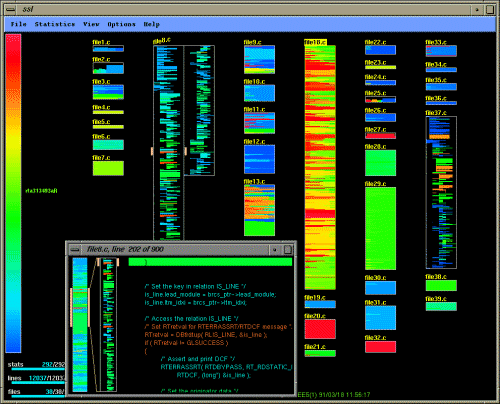
\includegraphics[width=0.8\linewidth]{Eick1992_Seesoft.png}
    \caption{Seesoft}
  \endminipage\hfill
  \minipage{0.5\textwidth}
    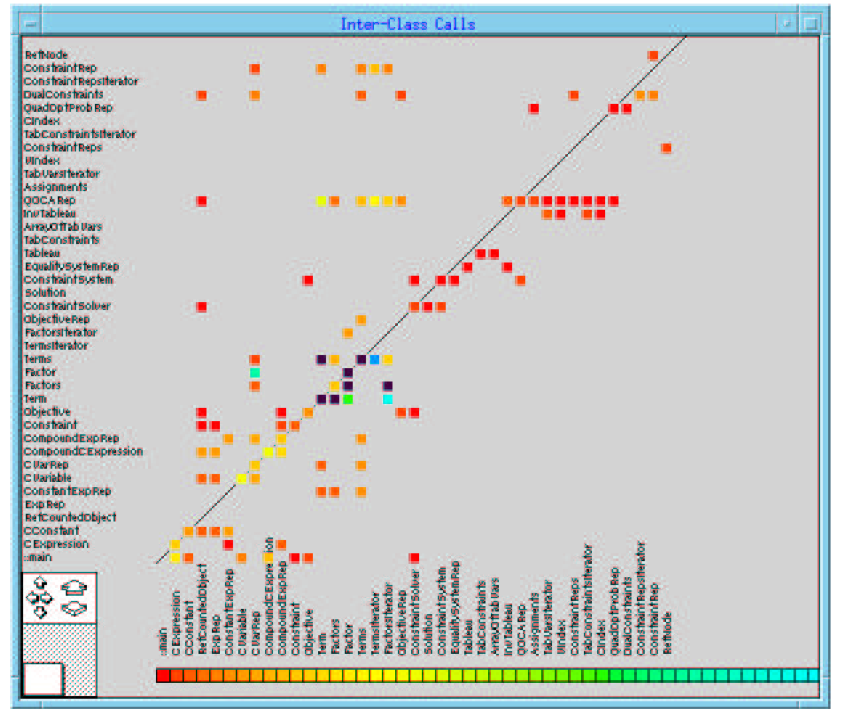
\includegraphics[width=0.8\linewidth]{DePauw1993_Jinsight.png}
    \caption{Jinsight}
  \endminipage\hfill
\end{figure}

% the first contributors to software evolution visualization were Holt and Pak in 1996, who used their tool called GASE [HP96]
% 		GASE: visualizing software evolution-in-the-large 

That period was favorable also for experimenting with novel research directions for visualization, 
such as 3D visualization and Virtual Reality. 


% In 1995, Reiss presented a configurable engine for building 3D visualization of programs called PLUM
\bigbreak
In 1998, Chuah and Erick \cite{Chuah1998} proposed three different techniques to visualize project data. 
They exploited the concept of glyphs, a graphical object that represents data through visual parameters. 
The first technique was the Timewhell glyph, used to visualize time-oriented information (number of lines of code, number of errors, number of added lines). 
The second technique was the 3D wheel glyph; it encoded the same attributes of the time wheel, and additionally, it used the height to encode time. 
Infobug glyph was the last technique, where each glyph was composed of four parts, each representing essential data of the system, such as time, code size, and the number of added, deleted, or modified code lines. \newline

\begin{figure}[H]
\minipage{0.32\textwidth}
  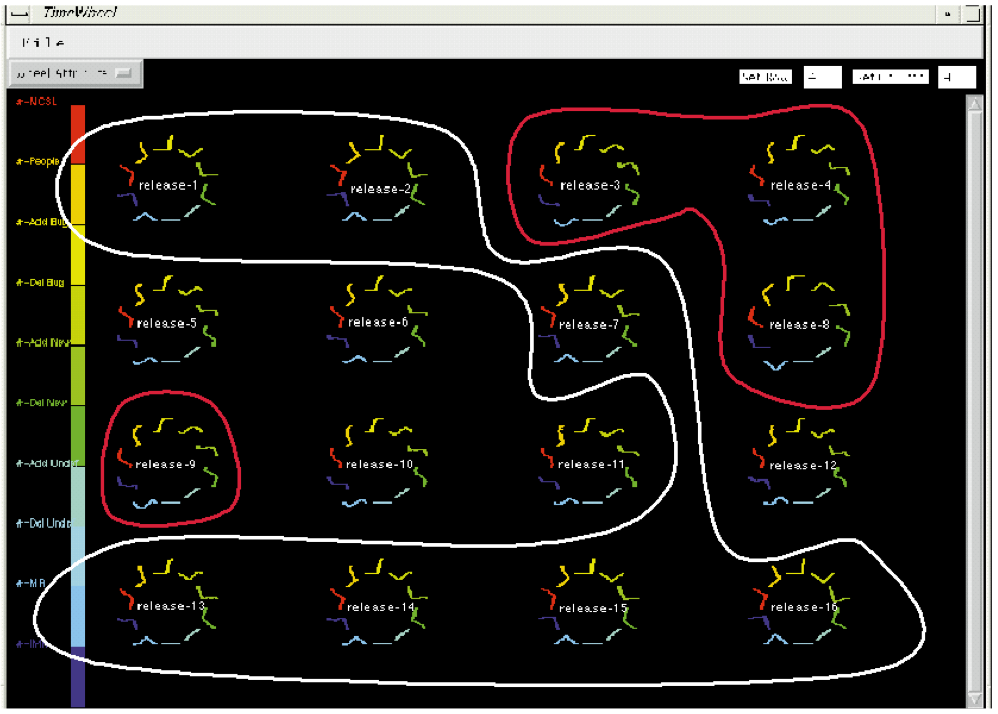
\includegraphics[width=\linewidth]{Chuan1.png}
  \caption{Timewhell}
\endminipage\hfill
\minipage{0.32\textwidth}
  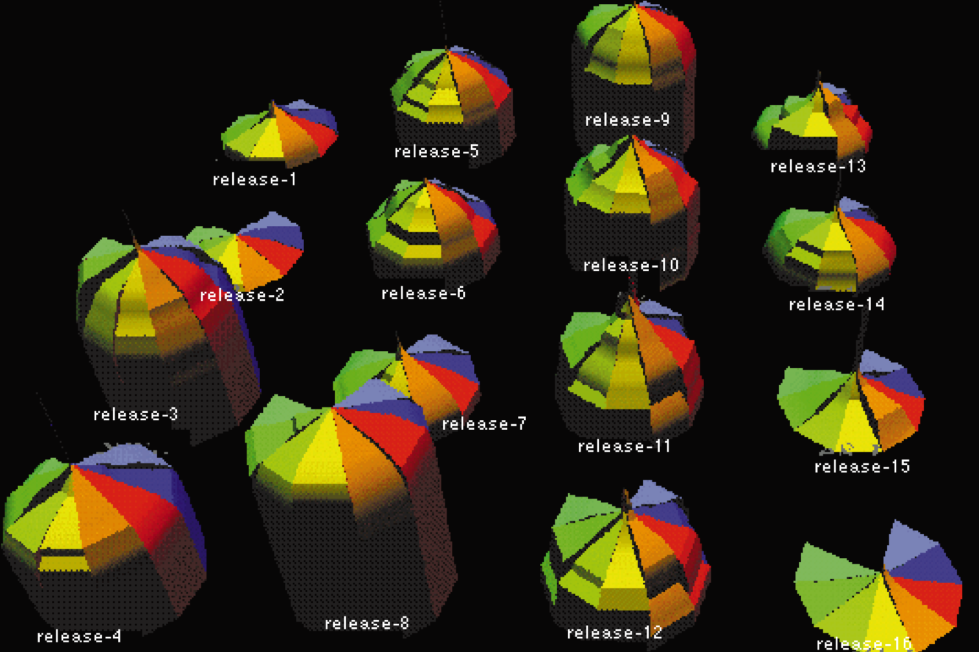
\includegraphics[width=\linewidth]{Chuan2.png}
  \caption{3D wheel}
\endminipage\hfill
\minipage{0.32\textwidth}%
  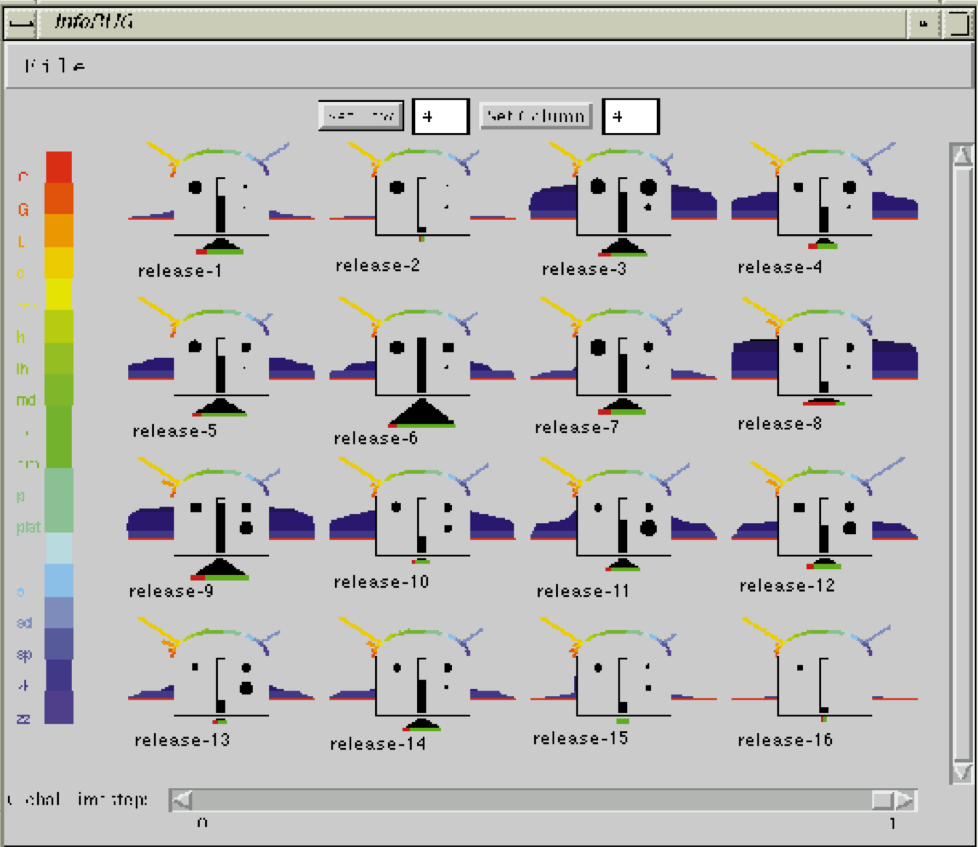
\includegraphics[width=\linewidth]{Chuan3.png}
  \caption{Infobug}
\endminipage
\end{figure}
 
\bigbreak
Also in 1998, Young and Munro \cite{Young1998} explored representations of software for program comprehension in VR. 

\bigbreak
Finally, in 1999, Jacobson et al. \cite{Jacobson1999} introduced what we now know as de facto the standard language to visualize the design of a system: UML. 


% Edward Tufte has influenced the entire field of information visualization, including software visualization.
% 	[Tuf90] Edward Tufte. Envisioning Information. Graphics Press, 1990.
% 	[Tuf97] Edward Tufte. Visual Explanations. Graphics Press, 1997.
% 	[Tuf01] Edward Tufte. The Visual Display of Quantitative Information. Graphics Press, 2nd edition, 2001.

% \subsection{Software evolution visualization}
%https://www.inf.usi.ch/faculty/lanza/Downloads/Gall2006a.pdf
\bigbreak
Before the beginning of the 21st century, thanks to the spread of version control systems and the open-source movement, 
visualizing the evolution of a system became a more feasible activity since there was more publicly accessible system information.   
As a result, many researchers focused their work on software evolution visualization.

\bigbreak
Lanza \cite{Lanza2001} introduced the concept of the Evolution Matrix. 
It was a way to visualize the evolution of software without dealing with a large amount of complex data. 
Furthermore, this approach was agnostic to any particular programming language. 
The Evolution Matrix aimed to display the evolution of classes in object-oriented software systems. 
Each column represented a version of the software; each row represented a different version of the same class.
Cells were filled with boxes whose size depended on evolutionary measurements. 
The shape of the matrix could also be used to infer various evolutionary patterns.

\begin{figure}[H]
\minipage{0.49\textwidth}
  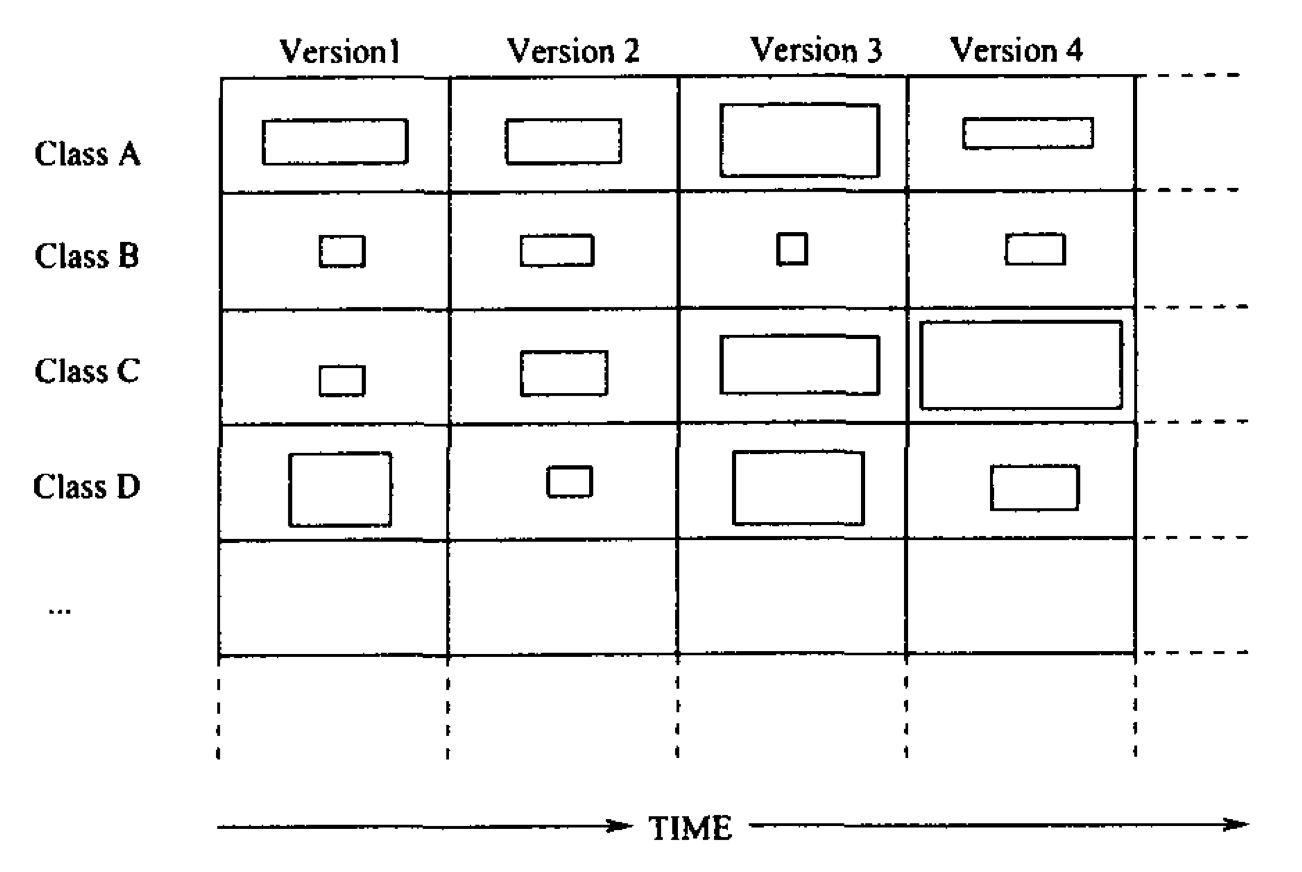
\includegraphics[width=\linewidth]{EvolutionMatrix1.png}
  \caption{A schematic display of the Evolution Matrix}
\endminipage\hfill
\minipage{0.49\textwidth}
  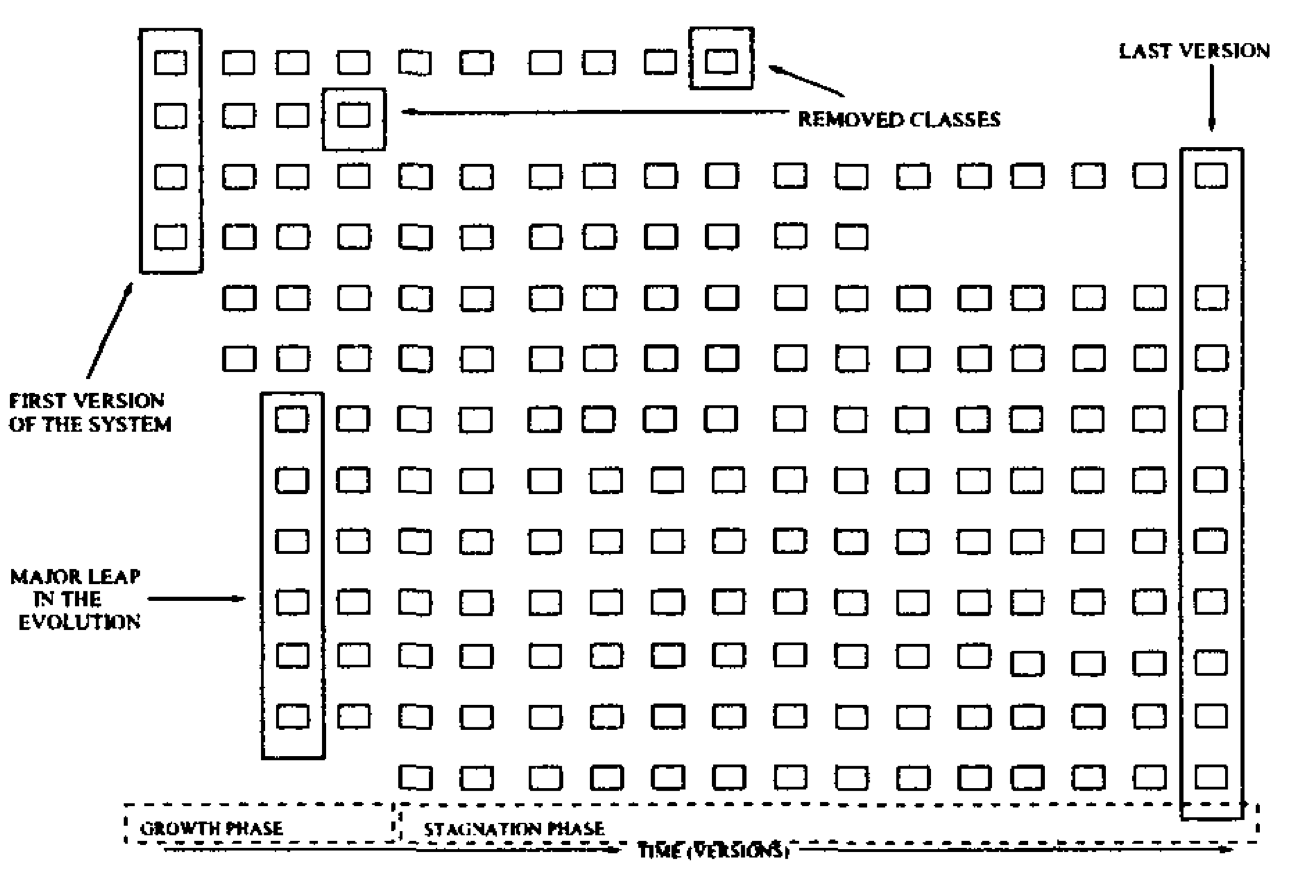
\includegraphics[width=\linewidth]{EvolutionMatrix2.png}
  \caption{Some characteristics of the Evolution Matrix}
\endminipage\hfill
\end{figure}

\bigbreak
Taylor and Munro \cite{Taylor2002},  demonstrated that it was possible to use the data contained in a version control repository to visualize the evolution of a system.
They developed Revision Tower, a tool that showed change information at the file level. 
Pinzger et al. \cite{Pinzger2005} visualized the evolution of a software system through Kivat diagrams.
RelVis, their tool, was able to depict a multivariate visualization of the evolution of a system.

\bigbreak
During the same year, Ratzinger et al. presented EvoLens \cite{Ratzinger2005}, a visualization approach and tool to 
explore evolutionary data through structural and temporal views.

\bigbreak
Langelier et al. \cite{Langelier2005} investigated the interpretation of a city metaphor 
\cite{Knight2000} to add a new level of knowledge to the visual analysis.
 
\bigbreak
D’Ambros and Lanza \cite{DAmbros2006} introduced the concept of Discrete-Time Figure concept. It was a visualization technique that embedded both historical and structural data in a simple figure. 
Their approach depicted relationships between the histories of a system and bugs. 
They also presented the Evolution Radar \cite{DAmbros2006a}, a novel approach to visualize module-level and file-level logical coupling information.

\begin{figure}[H]
  \minipage{0.33\textwidth}
    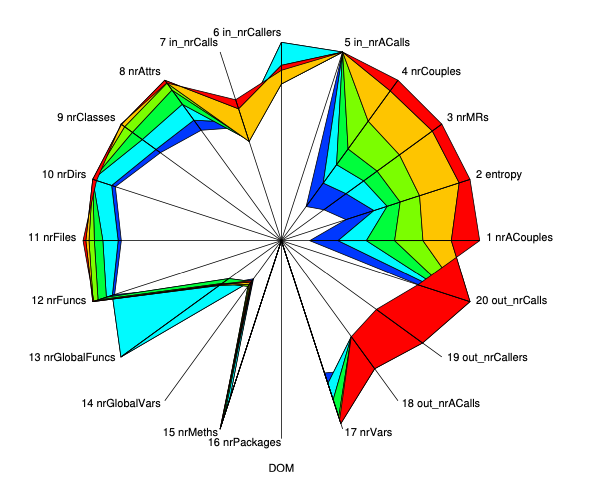
\includegraphics[width=\linewidth]{Pinzger2005_RelVis.png}
    \caption{RelVis}
  \endminipage\hfill
  \minipage{0.33\textwidth}
    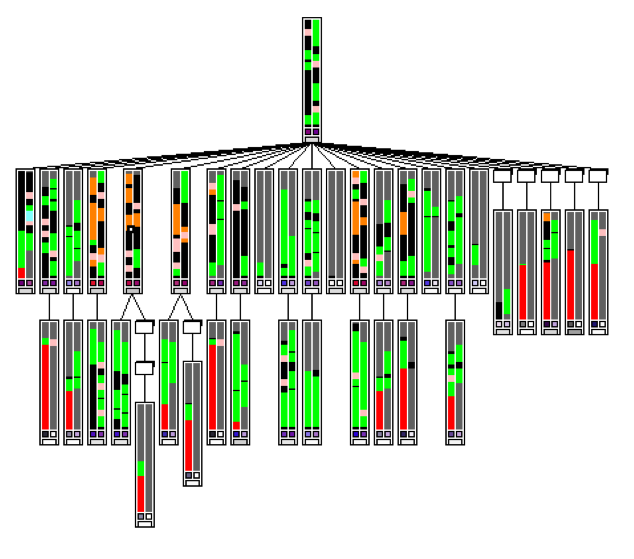
\includegraphics[width=\linewidth]{DAmbros2006.png}
    \caption{Tree of Discrete Time Figures}
  \endminipage\hfill
  \minipage{0.33\textwidth}
  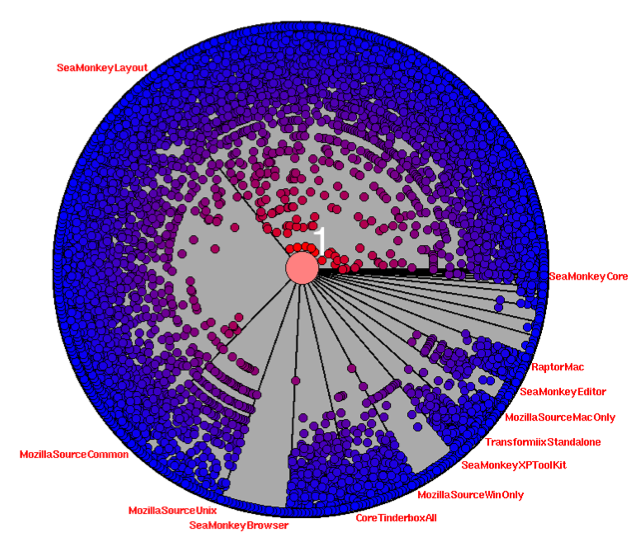
\includegraphics[width=\linewidth]{DAmbros2006a_EvoRadar.png}
  \caption{Evolution Radar}
\endminipage\hfill
  \end{figure}
  
  \bigbreak
Steinbrückner and Lewerentz \cite{Steinbrueckner2010} described a three-staged visualization approach to visualize large software systems. 
Thir visualization was supported by a tool called Evo-Streets. 
Each stage of their approach was responsible for representing a different aspect of the system with the city metaphor. 


\begin{figure}[H]
  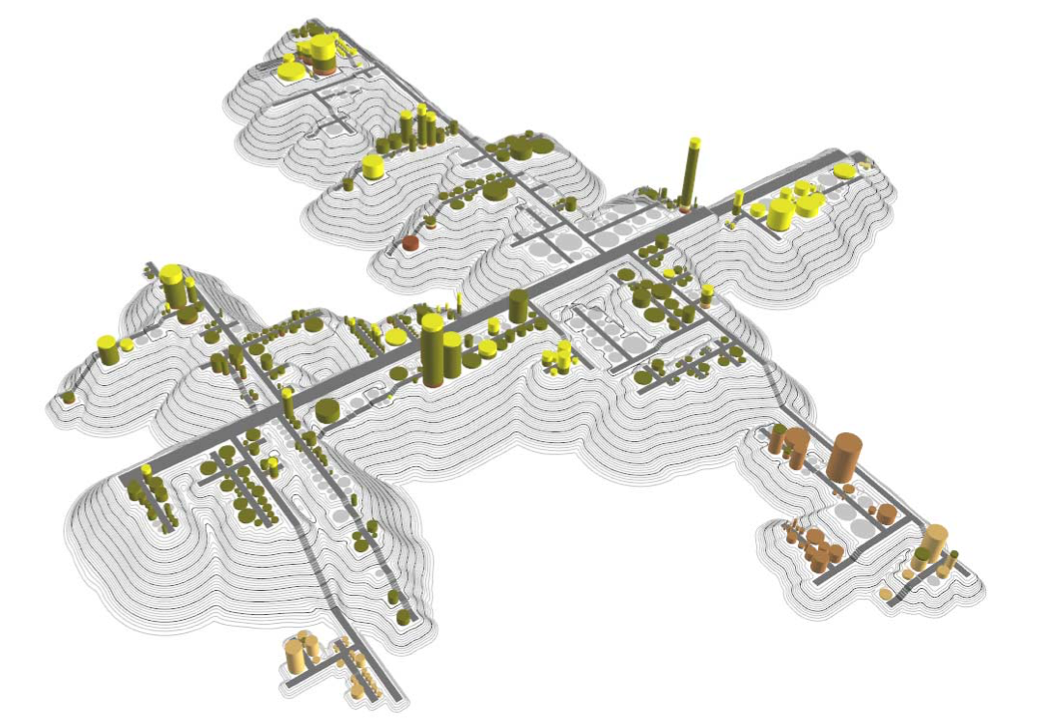
\includegraphics[width=0.9\linewidth]{Steinbrueckner2010.png} 
  \caption{Evo-Streets}
\end{figure}
 
\bigbreak
Wettel revised the city metaphor to represent metrics meaningfully  \cite{Wettel2011}. 
In his thesis, he represented packages as districts and classes as buildings.
The metaphor was used for various purposes, e.g., reverse engineering, program comprehension, software evolution, or software quality analysis. 
He claimed that the city metaphor brought visual and layout limitations; for example, not all visualization techniques fit well.
Under those circumstances, he preferred simplicity over the accuracy,
so he obtained a simple visual language that facilitated data comprehension. His approach was implemented as a software visualization tool 
called CodeCity. 


\begin{figure}[H]
  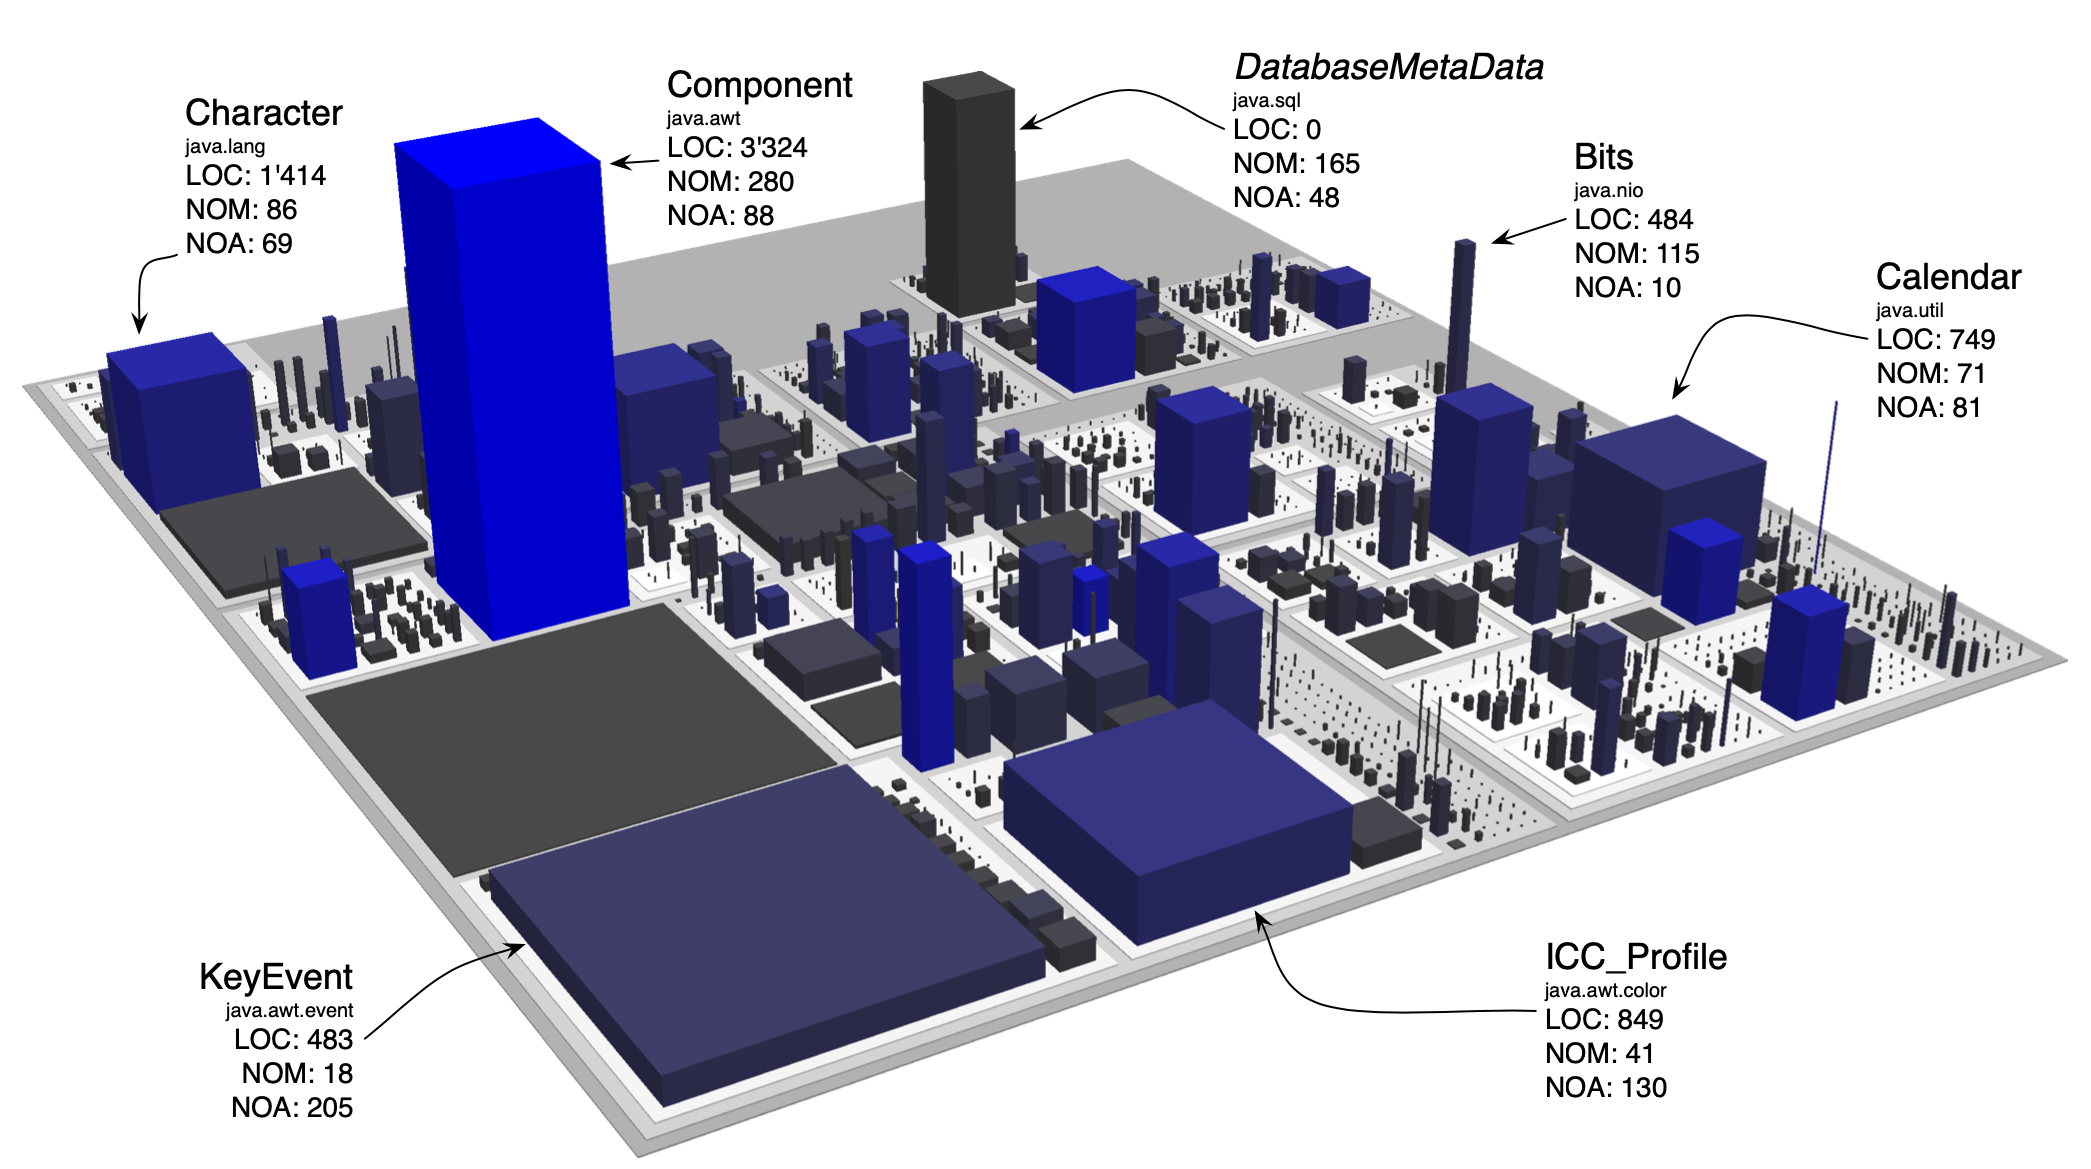
\includegraphics[width=0.9\linewidth]{CodeCity.png} 
  \caption{CodeCity}
\end{figure}

% TODO https://ieeexplore.ieee.org/document/1334769


% ChronoTwigger 2014 https://ieeexplore.ieee.org/abstract/document/6980223
\bigbreak
Ens et al. \cite{Ens2014} applied visual analytics methods to software repositories.
His approach helped users comprehend co-evolution information by visualizing how source and test files were developed together. 
 
% NN 2015 https://ieeexplore.ieee.org/document/7329727
\bigbreak
Kapec et al. \cite{Kapec2015} proposed a graph analysis approach with augmented reality. 
They made a prototype of a tool that provided a graph-based visualization of software, and then they studied some interaction methods to control it with augmented reality.
 
% CuboidMatrix 2016 https://ieeexplore.ieee.org/document/7780168
\bigbreak
Schneider et al. \cite{Schneider2016} presented a tool, CuboidMatrix, that employed a space-time cube metaphor to visualize a software system. 
A space-time cube is a well-known 3D representation of an evolving dynamic graph. 
 
% CityVR 2017 https://ieeexplore.ieee.org/abstract/document/8094470
\bigbreak
Merino et al. \cite{Merino2017} aimed to augment software visualization with gamification. 
They introduced CityVR, a tool that displays a software system through the city metaphor with a 3D environment. 
Working with virtual reality, they scaled the city visualization to the physically available space in the room. 
Therefore, developers needed to walk to navigate the system. 

\begin{figure}[H]
  \minipage{0.32\textwidth}
    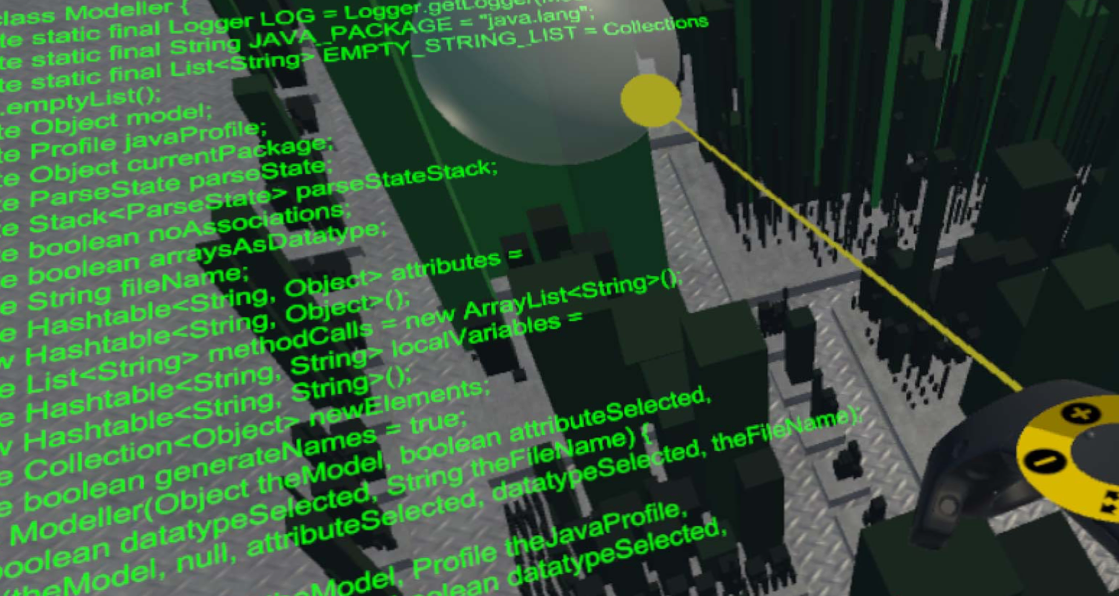
\includegraphics[width=\linewidth]{CityVR.png}
    \caption{CityVR}
  \endminipage\hfill
  \minipage{0.32\textwidth}
    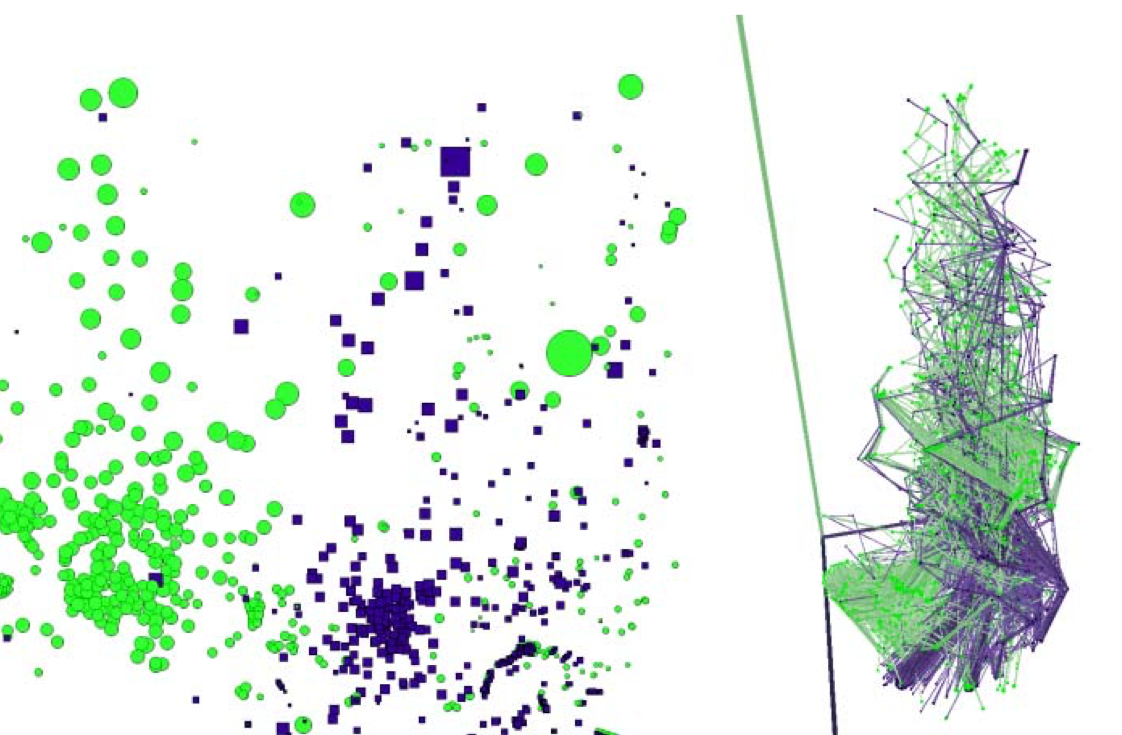
\includegraphics[width=\linewidth]{ChronoTwigger.png}
    \caption{ChronoTwigger}
  \endminipage\hfill
  \minipage{0.32\textwidth}%
    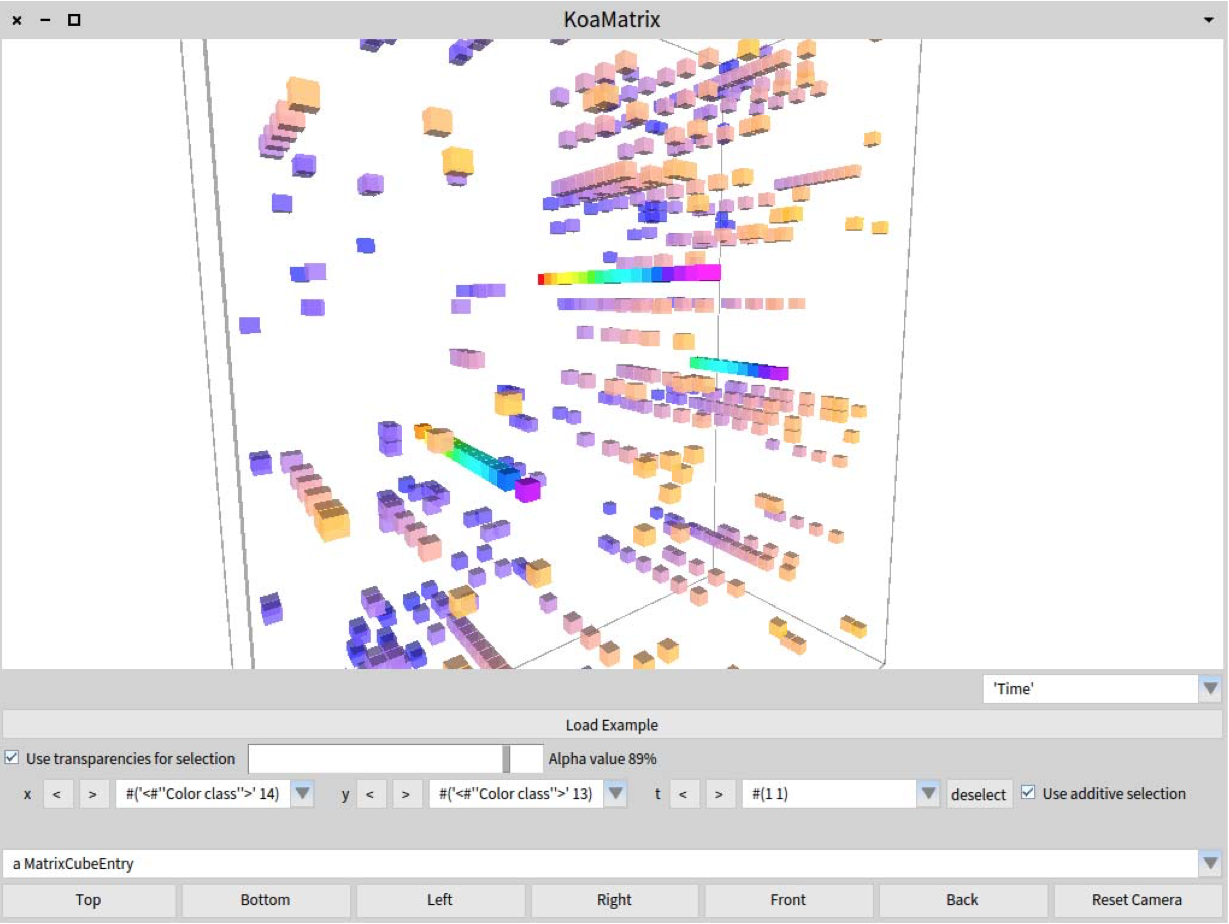
\includegraphics[width=\linewidth]{CuboidMatrix.png}
    \caption{CuboidMatrix}
  \endminipage
  \end{figure}
  


% Code Park 2017 https://ieeexplore.ieee.org/abstract/document/8091185
\bigbreak
Khaloo et al. \cite{Khaloo2017} revised the idea of gamification with a 3D park-like environment. They mapped each class in the codebase with a facility. The wall structure depended on constituent parts of the class e.g., methods and signatures. 

% Evo-Clocks 2019 https://ieeexplore.ieee.org/document/8900965
\bigbreak
Finally, we mention Alexandru et al., who proposed a method to visualize software structure and evolution, 
with reduced accuracy and a fine-grained highlighting of changes in individual components \cite{Alexandru2019}. 

\begin{figure}[H]
  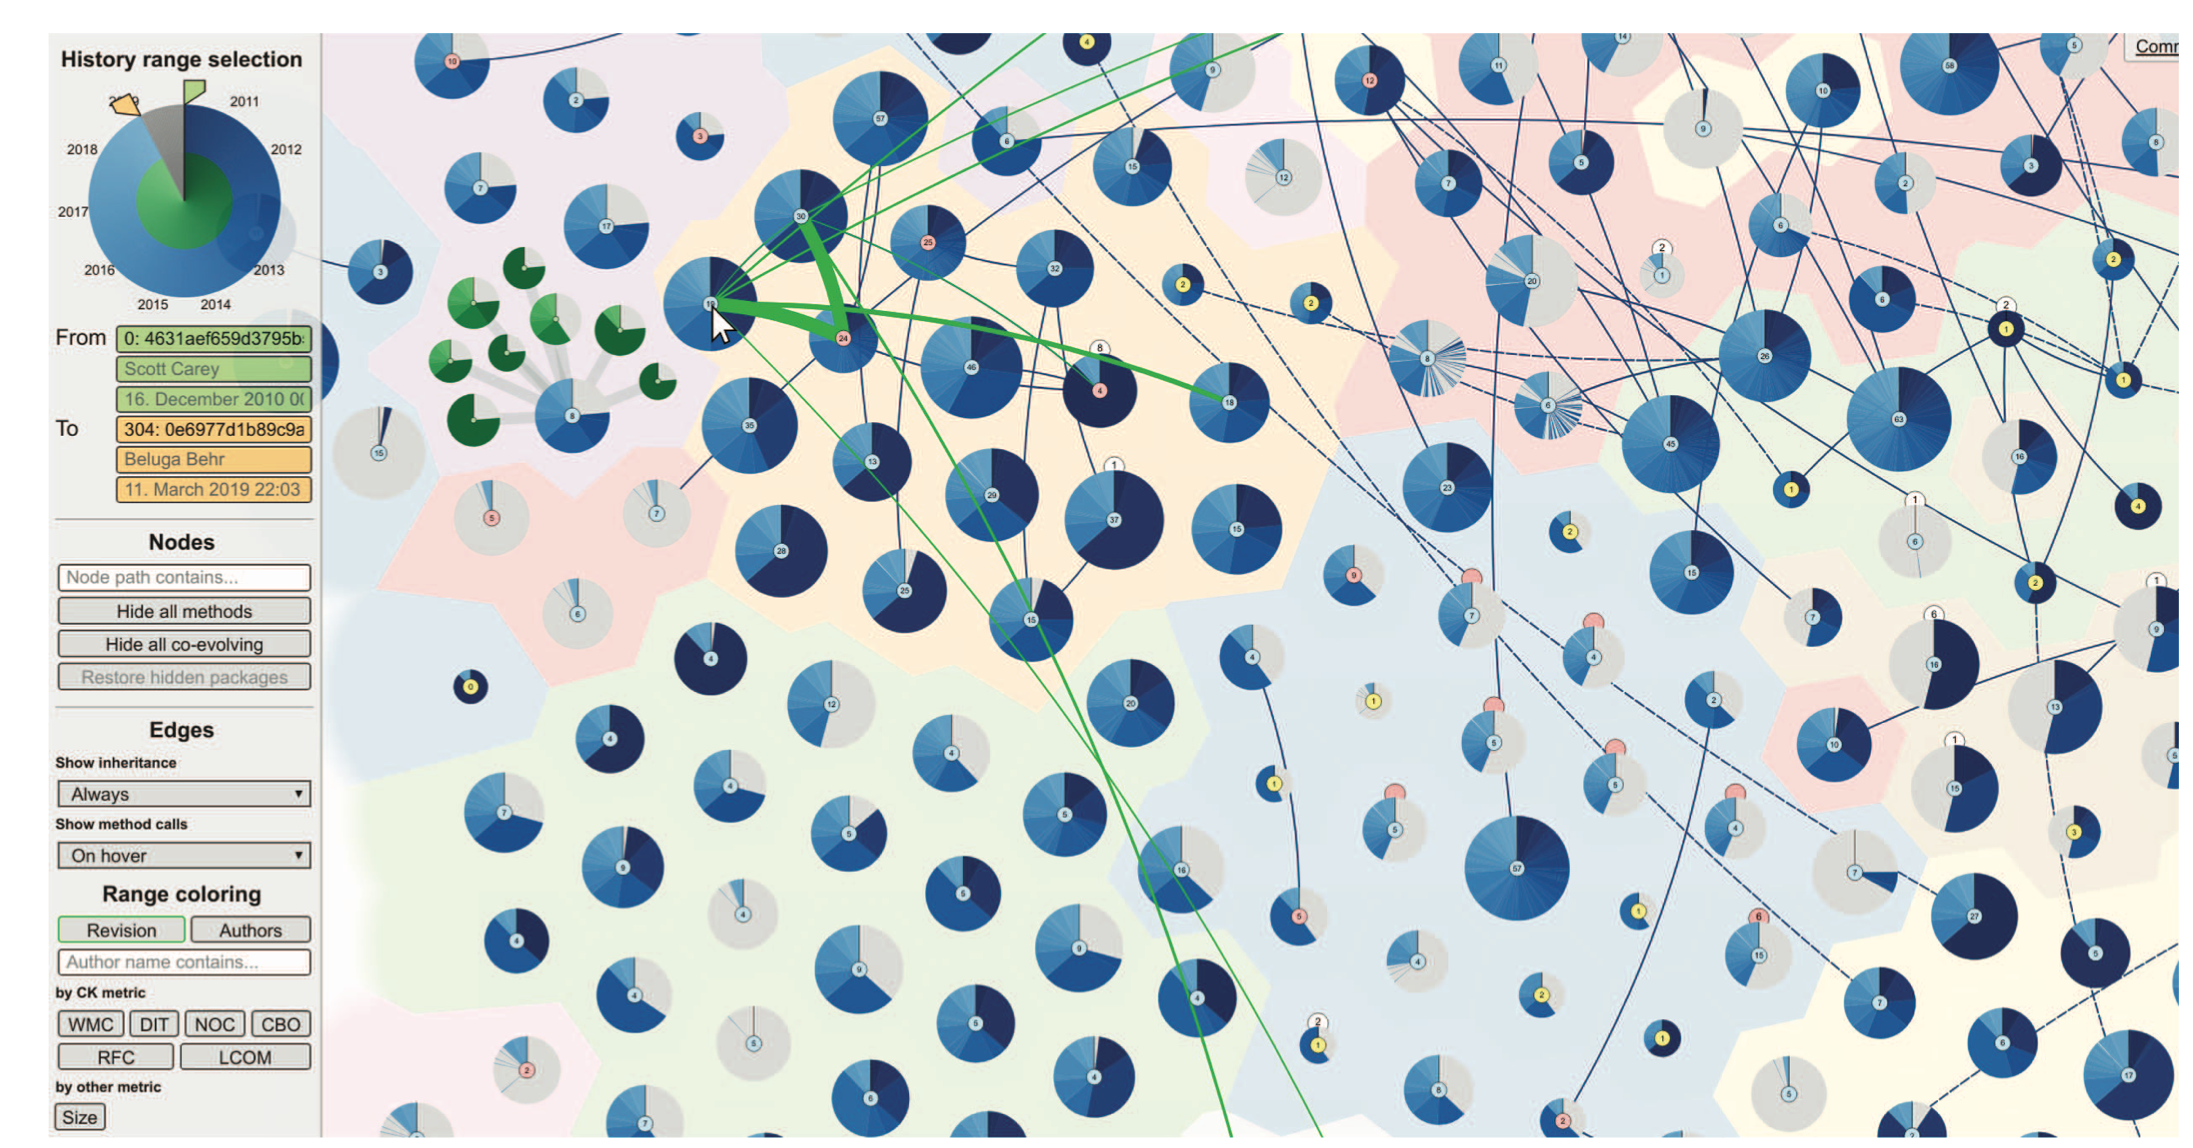
\includegraphics[width=0.9\linewidth]{Alexandru_EvoClock.png} 
  \caption{Evo-Clock}
\end{figure}


\section{Analysis of software evolution}

Software repositories contain historical data about the evolution of a software system. 
Thanks to the spread of the git protocol, and consequently of GitHub, 
Mining Software Repositories (MSR) has become a popular research field. 

\bigbreak
D'Ambros et al. in \cite{SoftwareEvolution} presented several analysis and visualization techniques to understand software evolution. 
They developed an approach based on a Release History Database (RHDB). 
In essence, it is a database that stores historical information about source code and bugs. 
The strength of RHDB was the association between historical versions of flies and bugs. 
Having this information stored on a database, they were able to run some evolution analysis to obtain information such as how many developers worked on a file to fix a bug or how was the effort to fix it.  

Finally, they concluded by evidencing two main challenges in MSR:
\begin{itemize}
  \item Technical challenge: repositories contain a sheer amount of data, and this poses scalability problems. 
  \item Conceptual challenge: how to do something meaningful with the collected data. 
  Most of the approaches present in literature to visualize software evolution have unanswered questions about the effectiveness of the comprehension. 
\end{itemize}

\begin{figure}[H]
  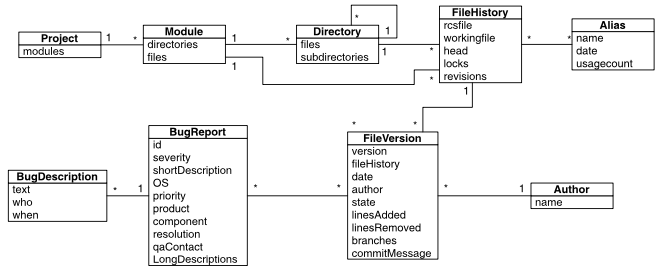
\includegraphics[width=0.9\linewidth]{RHDB.png} 
  \caption{RHDB}
  \label{fig:RHDB}
\end{figure}
 


% The promises and perils of mining GitHub  https://dl.acm.org/doi/abs/10.1145/2597073.2597074
\bigbreak
In 2022, the number of GitHub repositories lays around 200 million.
Even if it seems a promising source of data, Kalliamvakou et al. raised some issues with its mining. \cite{Kalliamvakou2014} 
For example, they evidenced that a repository does not always match with a project. 
A reason for this can be found in the fact that most repositories had had very few commits before becoming inactive.
When they made their research, over 70 percent of the GitHub projects were personal, and some of them weren't used for software development. 
Finally, the last perils that they raise, were related to GitHub features that are not properly used by software developers.
They considered only projects with a good balance between the number of commits, 
the number of pull requests and the number of contributors to find actively developed repositories. 
 

% PyDriller https://dl.acm.org/doi/abs/10.1145/3236024.3264598
\bigbreak
Spadini, Aniche and Bacchelli \cite{Spadini2018}. They developed a Python framework called PyDriller, enabling users to mine software repositories. 
Their tool can be used to extract information about the evolution of a software system from any git repository.  

\bigbreak
We also mention the work done by Salis and Spinellis \cite[]{Salis2019}.
They introduced RepoFS, a tool that allows navigating a git repository as a file system. 
Their approach sees commits, branches, and tags as a separate directory tree. 
Figure \ref{fig:RepoFS} shows an example of a repository data structure. 

\begin{figure}[H]
  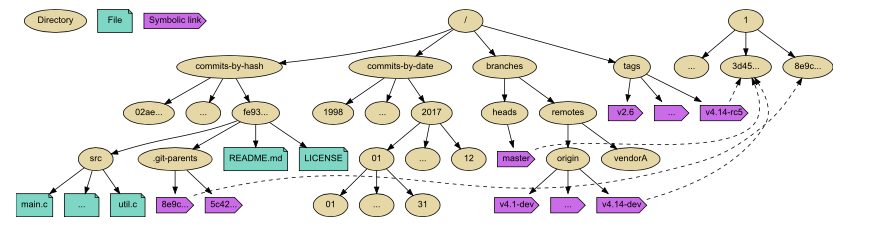
\includegraphics[width=0.9\linewidth]{Salis2019.png} 
  \caption{RepoFS}
  \label{fig:RepoFS}
\end{figure}

\bigbreak
Clem and Thomson \cite[]{Clem2021}, members of the semantic code team at GitHub, built a static analyzer of repositories to implement symbolic code navigation. 
That feature was released on GitHub some years ago and lets developers click on a name identifier to navigate to the definition of that entity. 
They were looking for a solution that would not bring them scalability problems. 
Moreover, they built the symbolic navigation feature around some ideas like:
\begin{itemize}
  \item Zero configuration needed by the owner of a repository
  \item Incrementality of the process. There was no need to process the entire repository for every commit made by a developer. Instead, they analyzed only the files that had changed. 
  \item Language agnosticism of the static analysis. 
\end{itemize}

Working on that feature, they recognized the difficulty of scaling a static analysis like that regarding human behavior. 
Nevertheless, their idea was to have an agnostic static analyzer, they cannot reach this goal and they were forced to implement it for just nine programming languages.  

\section{Data sonification}

External auditory representations of programs (known as "program auralisation") is a research field that 
is getting even more interest in the recent years.

% InfoSound https://ieeexplore.ieee.org/document/205229
\bigbreak
Sonnenwald et al. made one of the first attempts. \cite{Sonnenwald1990}
They tried to enhance the comprehension of complex applications by playing music and special sound effects. 
This approach was supported by a tool called InfoSound
It was mainly adopted to understand the program's behavior. 

\bigbreak
Many other researchers followed this first technique. To cite some of them, DiGiano and Baecker \cite{DiGiano1993} made LogoMedia, a tool to associate non-speech
 audio with program events while the code is being developed. 
Jameson \cite{Jameson1994}] developed Sonnet, audio-enhanced monitoring and debugging tool.  
Alty and Vickers \cite{Vickers2003} had a similar idea. Using a structured musical framework, they could map the execution behavior of a program to locate and diagnose software errors. 
 
% EXTERNAL AUDITORY REPRESENTATIONS OF PROGRAMS https://smartech.gatech.edu/bitstream/handle/1853/50854/Vickers2004a.pdf?sequence=1&
\bigbreak
Despite the usefulness of these tools, they adopted an essential kind of mapping, and thus they had a limited musical representation. 
Vickerts \cite{Vickers2004} evidenced the necessity of a multi-threaded environment to enhance the comprehension given by the musical representation. 
He proposed adopting an orchestral model of families of timbres, to enable programmers to distinguish between different activities of different threads.

\bigbreak
The size and the complexity of systems can represent a problem for the effectiveness of a visual representation of a software system.
Having a large number of visual information, observers might find it difficult to focus only on the relevant aspects. 
% CocoViz https://ieeexplore.ieee.org/document/5070558
Boccuzzo and Gall \cite{Boccuzzo2009} supported software visualization with sonification. 
They used audio melodies to improve navigation and comprehension of their tool, called CocoViz.
Their ambient audio software exploration approach, exploited audio to intuitively describe the position of an entity in the space. 
Thanks to the adoption of surround sound techniques, the observers perceived the origin of an audio source so, it could adjust his navigation in the visualization.
Each kind of entity played a different sound, based on mapping criteria.

\begin{figure}[H]
  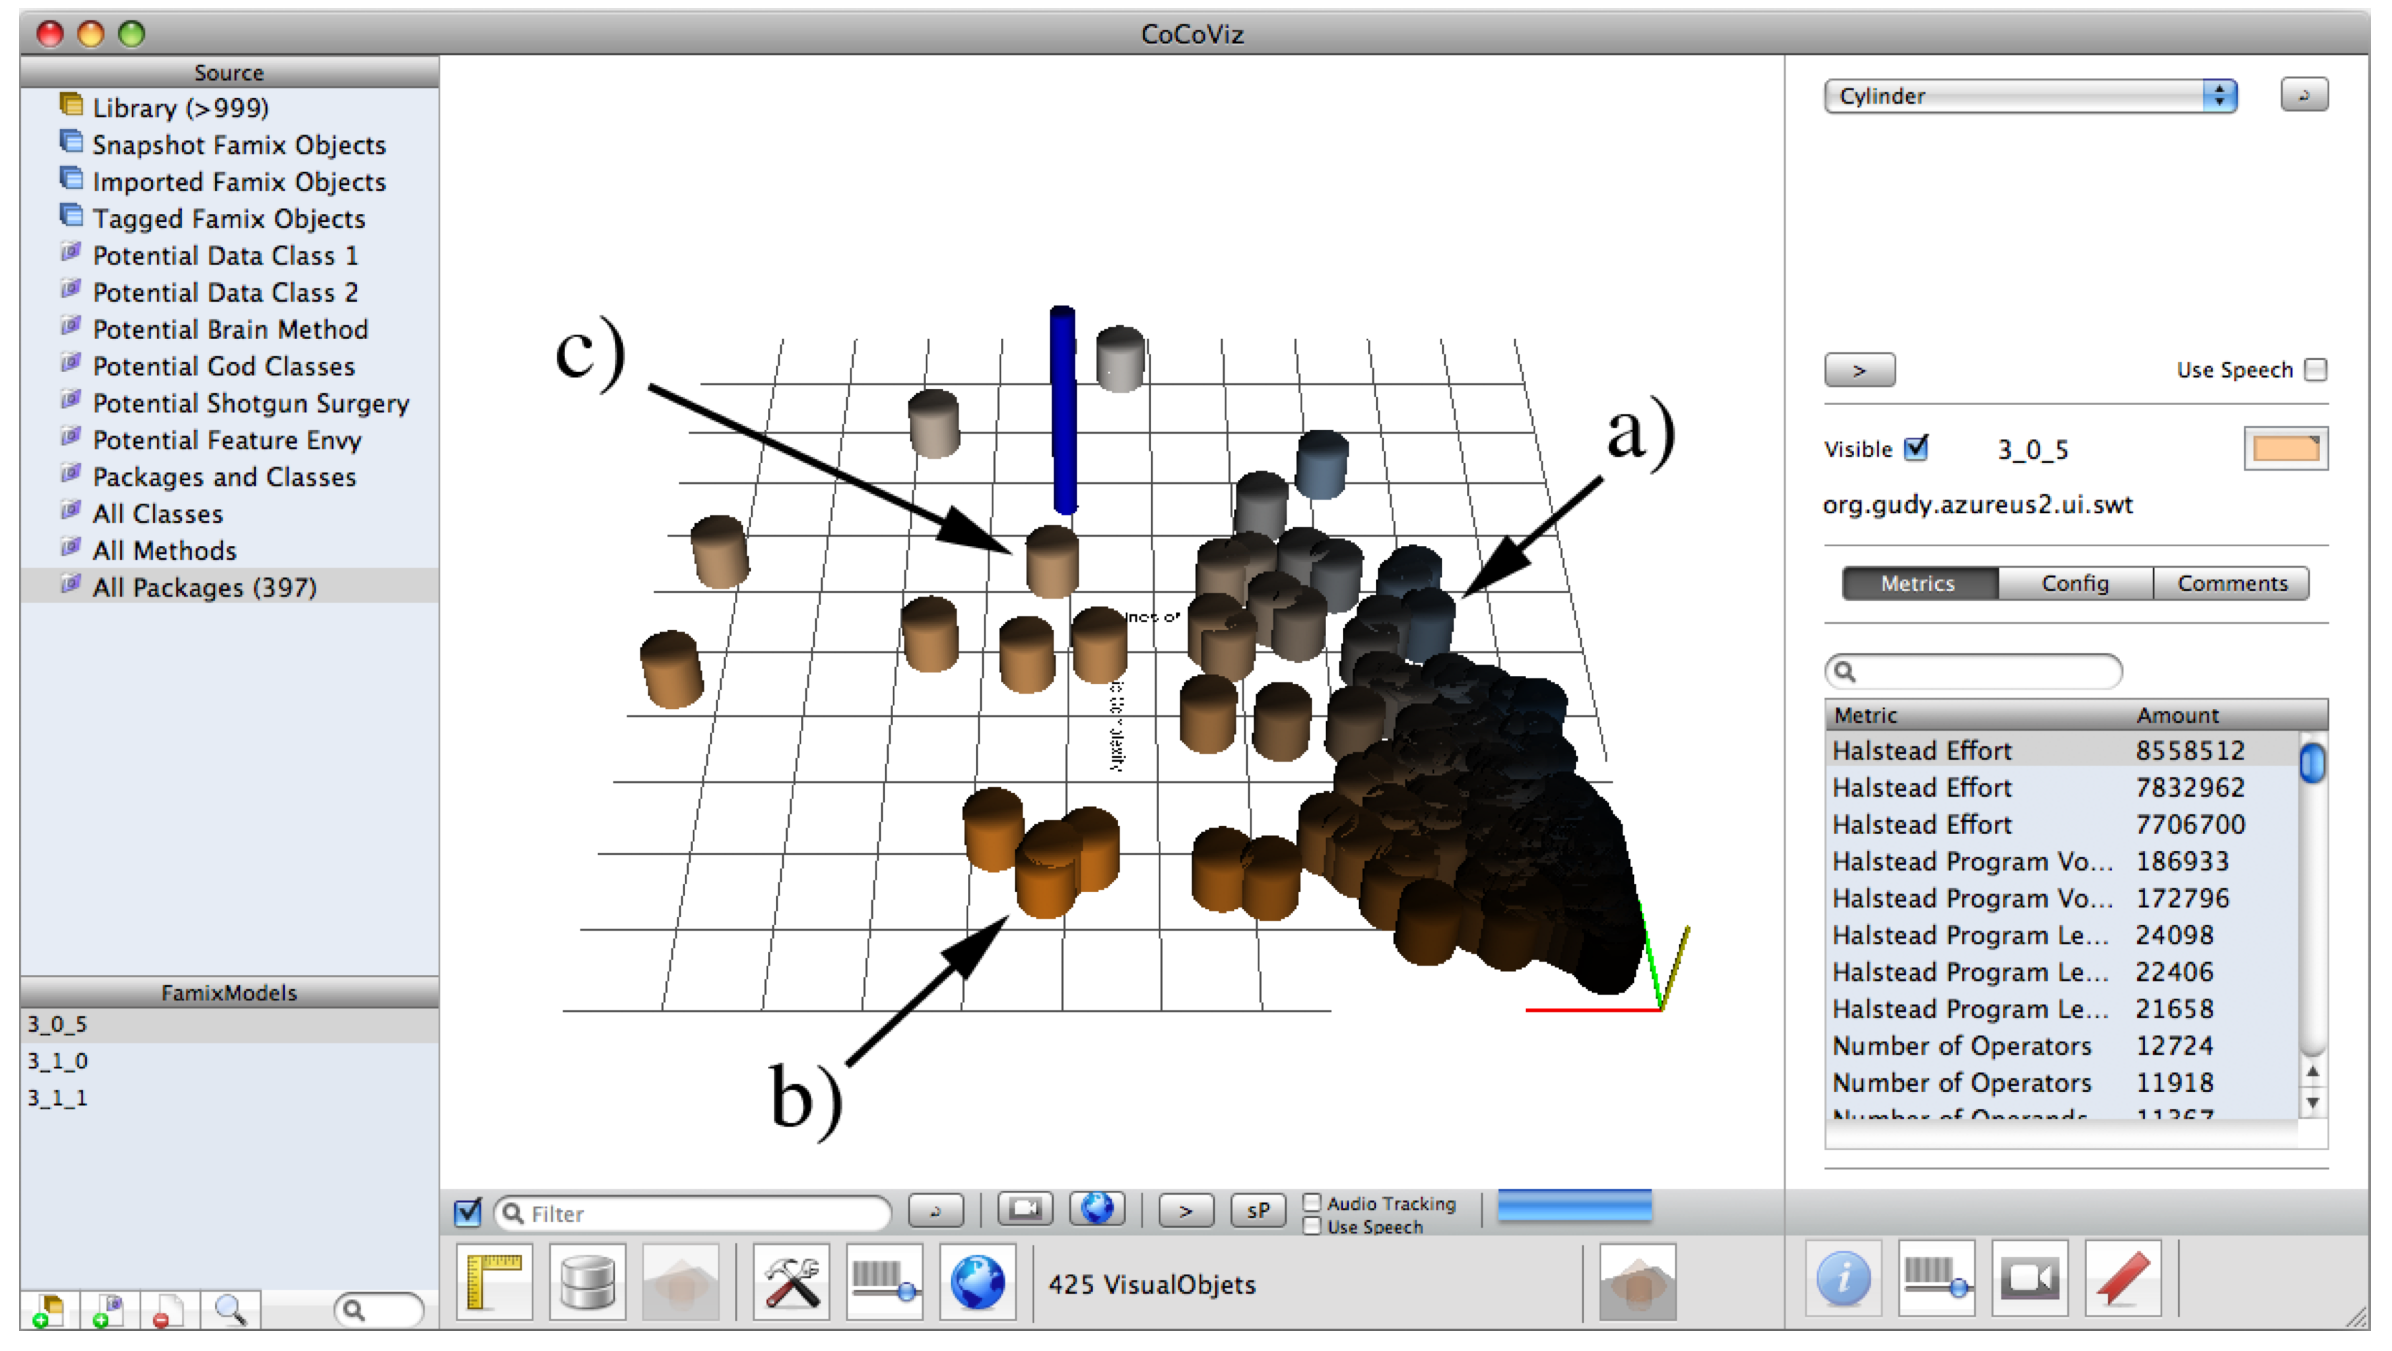
\includegraphics[width=0.9\linewidth]{CocoViz.png} 
  \caption{CocoViz}
\end{figure}


 
% Orchestrating change: An artistic representation of software evolution https://ieeexplore.ieee.org/document/6747192 
\bigbreak
McIntosh et al. \cite{McIntosh2014} explored the use of a parameter-based sonification, to produce a musical interpretation of the evolution of a software system.
Their technique mapped musical rests to an inactive period of development and consonance and dissonance to interesting phenomena (like co-changing of components).
% Software Musification https://ieeexplore.ieee.org/document/8107958
\bigbreak
Finally, Mancino and Scanniello \cite{Mancino2017} presented an approach to transforming source code metrics into a musical score that can be both visualized and played. 


\section{Conclusion}

We have seen many different approaches and tools focused on the visualization of one aspect of the system. Many of them were focused on some metrics and conversely many of them were focused on their evolution. 
Our approach is not based on a previously identified and well-known metaphor, such as CodeCity or CityVR. We aim to mine software repositories versioned with git and to find a suitable model to represent its history. 
Moreover, with this goal, we are aware of the scalability involved with MSR. Nonetheless, we will try to run a static analysis on the most relevant repositories, in terms of size, on GitHub. 
Our goal is to provide a fully language-agnostic static analyzer, despite what the GitHub team did on their work. Although, our goal is to visualize the evolution of a repository, not to semantically analyze the source code. 
Most of the visualization techniques used colors and shapes to enhance the strength of the comprehension. We aim to do the same but in a different way
Most of the visualization techniques used colors and shapes to enhance the strength of the comprehension. We aim to do the same but in a different way
Most of the visualization techniques used colors and shapes to enhance the strength of the comprehension. We aim to do the same but in a different way
Most of the visualization techniques used colors and shapes to enhance the strength of the comprehension. We aim to do the same but in a different way
Most of the visualization techniques used colors and shapes to enhance the strength of the comprehension. We aim to do the same but in a different way
Most of the visualization techniques used colors and shapes to enhance the strength of the comprehension. We aim to do the same but in a different way


%!TEX root = SYN.tex

\chapter[Approach]{Approach}
\graphicspath{ {images/approach} }

Comprehending the evolution of a software system is a complex activity, mainly because of the sheer amount of data and its complexity. 
The term \quotes{software evolution} was coined for the first time by Lehman in 1985 in a set of laws \cite{Lehman1985}.
He stated that the complexity of a system is destined to increase over time as the system needs to be adapted to its evolutionary environments. 
To be maintained, software systems need to be comprehended by developers, and this activity can be supported with software visualization. 

The development activity is often supported by a Version Control System (VCS) software for tracking and managing file changes. VCSs have been widely adopted for the last 40 years. Revision Control System (RCS) is one of the oldest, and it was introduced in 1980. Consequently, between 1990 and 2020, developers introduced several VCSs. The most important ones were Concurrent Versions System (CVS) introduced in 1990, Perforce (1995), Subversion (2000), Mercurial, and Git (2005).

One of the most adopted ones is Git, introduced in 2005 by Linus Torvalds\footnote{\url{https://github.com/git/git/commit/e83c5163316f89bfbde7d9ab23ca2e25604af290}}. Millions of repositories use it on GitHub and GitLab. 
For this reason, we focused on systems versioned with this protocol.
Git is a versioning control system that tracks all the changes made to every system file. 
Internally git holds all the information we need to reconstruct the history of a repository. 

In this chapter, we present our sensorial approach to visualizing a software system using a visual and auditive depiction of its evolution. 
To fulfill this purpose, we leverage synesthesia, the production of a sense impression relating to one sense by stimulation of another sense.
Moreover, we also present how we reconstruct and model the history of a repository. 

In this chapter, we present the three main steps of our approach as follows:
\begin{itemize}
    \item first, we model the system's evolution; 
    \item next, we visualize it;
    \item finally, complement the visualization with an auditive portrayal of evolutionary data. 
\end{itemize}

\newpage
\section{Evolution Model}
\label{s:EvolutionModel}

\begin{figure}[H]
    \begin{center}
        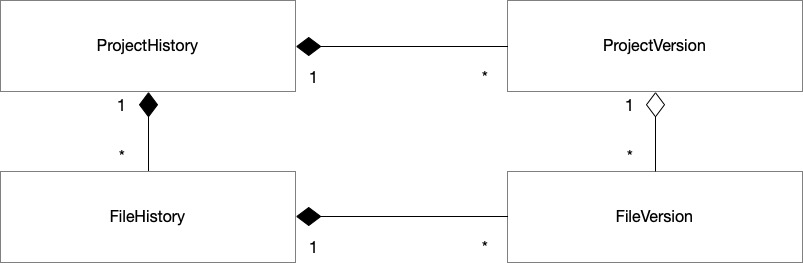
\includegraphics[width=0.6\textwidth]{EvolutionModel.jpg}
    \end{center}
    \caption{Evolutionary Model}
    \label{fig:EvolutionaryModel}
\end{figure}
Various approaches have been proposed to analyze aspects of software evolution. In 2005, Tudor Girba presented Hismo \cite{Girba2005}, a model centered around the notion of history as a first-class entity. Our approach is based on this work. The need to develop a novel evolutionary model comes from the fact that Hismo was designed to work with another versioning system: Subversion (SVN). 
There are several differences between SVN and git. In terms of design, the most important is how they track changes. 
SVN works with the concept of \quotes{snapshot} while git works with the concept of \quotes{commits}. In SVN, when a file has been changed, a new revision of the whole system is created, and consequently, the number of revisions is incremented. 
In contrast, in git, only the modified files would get committed, and thus we don't have a new snapshot of the system every time. 
Therefore, we took Hismo as the starting point of our model and adapted it to the git protocol. 
The Hismo model was based on three concepts:
\begin{itemize}
    \item Snapshot. A representation of the entity whose evolution is studied.
    \item Version. A representation of a system's version. It defines the time when a snapshot was made. 
    \item History. An entity that holds a set of Versions.
\end{itemize}

We replaced the concept of Snapshot with a FileVersion. It represents the version of a file at a particular point in time. Instead of being related to every version of the system, it is related only to the Versions when the file was updated.
Moreover, we made a distinction between File entities and Project entities. So, we mapped the concept of History to FileHistory and the idea of Version to ProjectVersion. 
The entity responsible for holding both of them is called ProjectHistory. \autoref{fig:EvolutionaryModel} depicts the relationships among these concepts. 
To summarize, these are the four main concepts of our evolutionary model: 
\begin{itemize}
    \item \textbf{ProjectHistory}: represents the history of a repository. It holds two sets: a set of FileHistories and a set of ProjectVersions. 
    \item \textbf{FileHistory}: represents a file inside the repository. We consider each file as an entity of the system. Even if the entity's name or location is changed, our model will treat it as the same. So, our approach is resilient to renaming and moving activities. Each FileHistory holds a set of FileVersions, each representing a different version of the entity at a particular point in time.  
    \item \textbf{ProjectVersion}: represents a commit or a version of the system. 
    For each changed file inside a commit, the respective ProjectVersion contains a FileVersion representing that change.
    A ProjectVersion holds contextual information about the commit, such as its timestamp, hash, and message.
    \item \textbf{FileVersion}: represents the version of a file at a particular point in time.
    It is responsible for holding all the evolutionary information of an entity, such as the last action on a file. 
\end{itemize}

\subsection{Historical information retrieval}
To model the history of a repository, we need to extract the historical information from git.
Git works with the concept of branches. Each branch can be seen as a different repository timeline.
Usually, developers use branches to develop features and merge the developed code in a branch that contains the stable codebase.
They create a \quotes{merge commit} to do that. 
Each time developers create a new git commit, they deploy a new version of the system that records all the changes made to the commits' tracked files. 
Internally, in git, all git stores all the commits as nodes of a commit-tree. 
The root node represents the repository's first commit and has no parents. 
All the other nodes represent the commits made during the whole lifecycle of the repository. 
Each commit usually has only one parent representing the previous commit.
There is one case where a commit might have more than one parent: merges commits.

Each repository should have a branch containing stable, production-ready code as a convention. Usually, this branch is named \quotes{main} or \quotes{master}. 
In our approach, we aim to analyze the timeline of this stable branch. We start from the root of the commit tree, which represents the initial commit, and then we traverse the whole tree. 
We do not consider \quotes{merge commits} during this process since they already incorporate previous commits, and thus they would be considered twice. 
Once we have extracted all the valid commits that reside on the stable branch, we need to extract all the representative information for a ProjectVersion. \\

Git can recognize the following file actions:
\begin{itemize}
    \item \textbf{ADD}. A file is added to the repository.
    \item \textbf{DELETE}. A file has been removed from the repository.
    \item \textbf{MODIFY}. The contents of a file have been modified.
    \item \textbf{RENAME}. A file's name has been changed but the file remained in the same parent directory.
    \item \textbf{MOVE}. A file was moved from one location to another. This action is detected whether the file's name remains the same. 
\end{itemize}

From a commit, we could also extract additional information such as the name of the file being modified, the action made on a file, the number of lines added and removed, and the file paths before and after the changes.
We used the commit's information to track all the paths of an entity. We can update the entity path when it was renamed or moved to follow it during its lifecycle. \\
%\linebreak
When we reconstruct the history of a repository, each FileHistory starts with a FileVersion representing an ADD action.
During the lifecycle of a repository, files can be deleted. In this case, the last FileVersion held by a deleted FileHistory represents a DELETE action.

\begin{figure}
    \begin{center}
        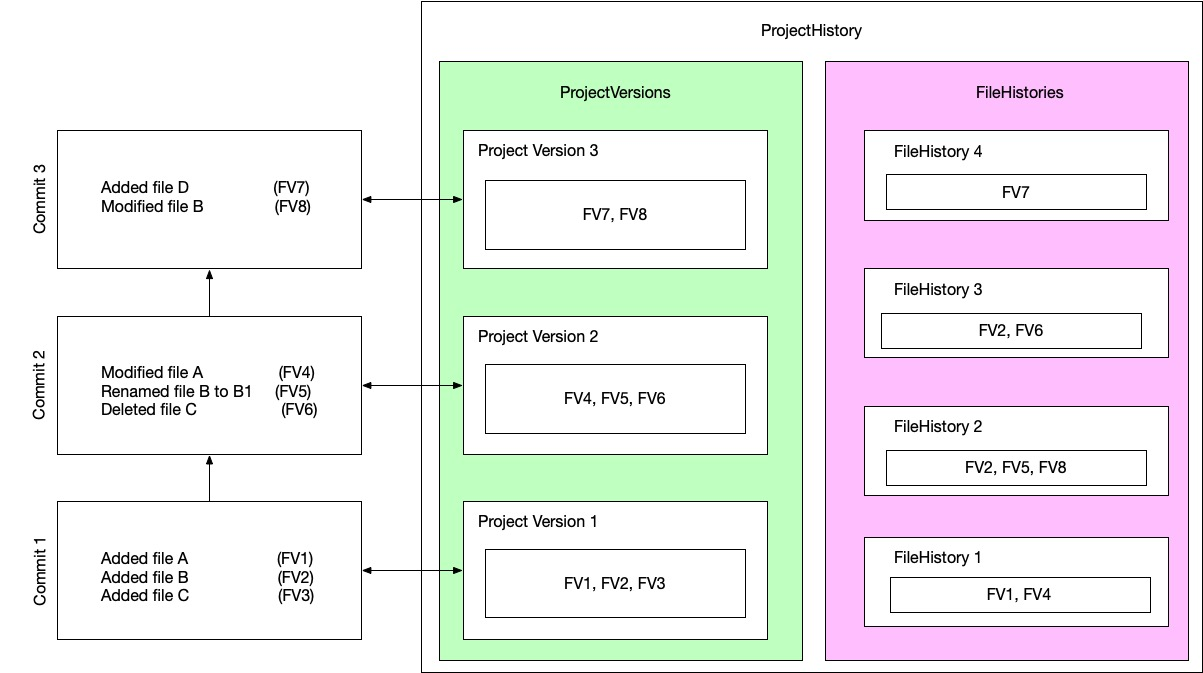
\includegraphics[width=0.8\textwidth]{RebuildingHistory.jpg}
    \end{center}
    \caption{Rebuilding history example}
    \label{fig:RebuildingHistory}
\end{figure}

\autoref{fig:RebuildingHistory} shows an example of building an instance of the evolution model.
First, we create a ProjectHistory with a set of ProjectVersions and a set of FileHistories.
After that, we start to traverse the repository's commit tree.
For each commit, we create a new ProjectVersion that represents a new version of the system. 
We inspect the commit's changelog and create a new FileVersion for each list entry.
Every time we find a newly added file in the changelog of a commit, we create a new FileHistory. 
In the example, in version 1, three new files were added to the repository (A, B, C). Thus, three new FileHistories were created.
Each change was mapped to a FileVersion (FV) and consequently added to the respective FileHistory and ProjectVersion. 
We did the same for ProjectVersions 2 and 3. 

\label{sec:partialHistoricalRepr}
\subsection{Partial historical representation}
\begin{figure}[ht]
    \begin{center}
        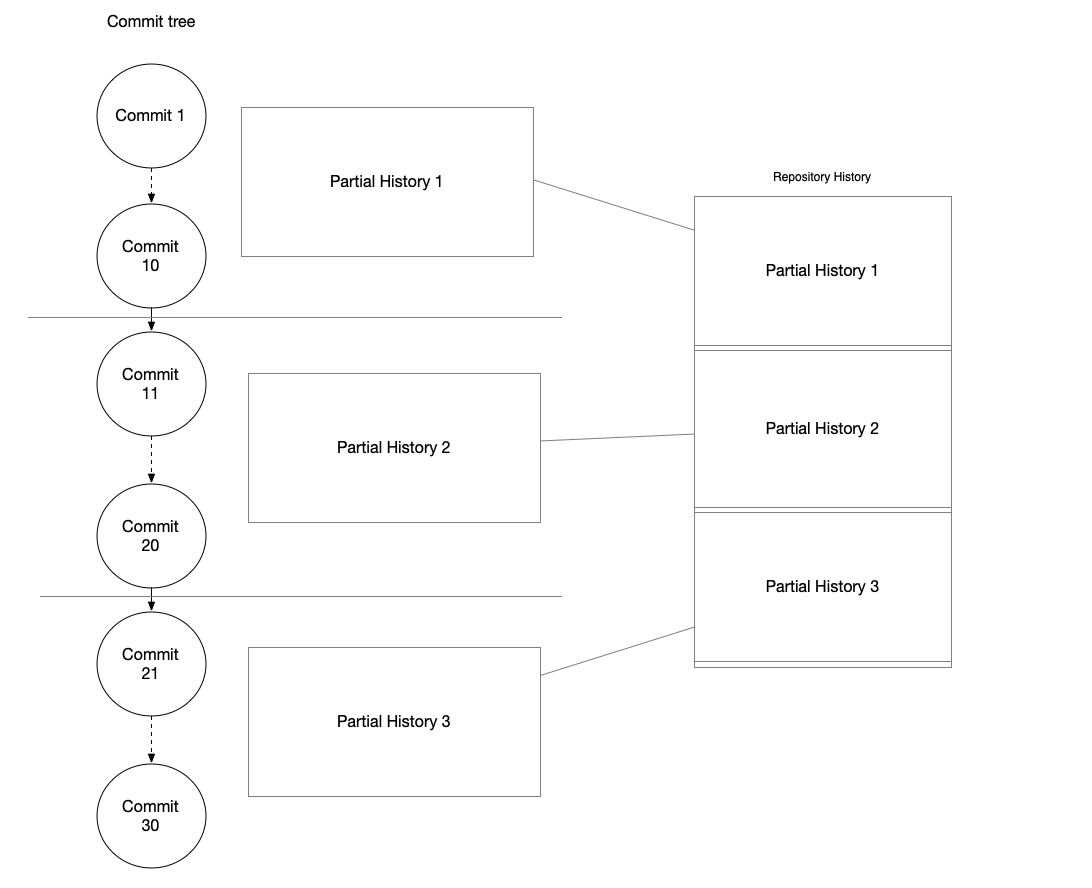
\includegraphics[width=0.5\textwidth]{PartialHistory.png}
    \end{center}
    \caption{Partial history example}
    \label{fig:PartialHistory}
\end{figure}
We had as a goal to develop a scalable approach to mine software repositories. This way, it should always be possible to analyze large repositories in an acceptable amount of time. 
In other words, our approach needs to be scalable.
GitHub host the code of some notorious open-source systems, such as LibreOffice, Elasticsearch, and Linux.
They all have more than 500,000 commits each. Thus, we cannot aim to reconstruct their histories with a single analyzer, as it would take too much time.  
At the time of writing, the repository of Linux had 1,090,563 commits. 
To checkout from one commit to another, we could assume that git needs one second. 
As a result, just to navigate through the whole history of Linux, we would need 11 days.
Moreover, in this simple estimation, we are omitting the time the analyzer needs to extract metrics from every file on each version. 

To overcome this mining issue, we present a scalable approach based on the concept of partial history.
A partial history holds information about a specific range of time of the ProjectHistory. 
It can be seen as a subset of a ProjectHistory. 
We can split the repository's history into multiple parts, each represented by a partial record. Then when all the analyses are completed, we merge them to reconstruct the whole story of the repository.


\autoref{fig:PartialHistory} shows an example PartialHistory representation. 
We split the commit tree into multiple chunks and then run the analysis on each. 
In the end, the final history will be represented by merging all the PartialHistories. 
Nonetheless, we can build PartialHistories in parallel, but we cannot do the same for the final History, 
because the final merge needs to be done sequentially. The sequence needs to follow the order of the commit tree. 
In \autoref{fig:PartialHistory}, for example,
Partial History 1 represents the history from commit 1 to commit 10, 
Partial History 2 represents the history from commit 11 to commit 20, and 
Partial History 3 represents the history from commit 21 to commit 30.
Therefore, the commit order is respected if we merge them in this order: 1, 2, 3. 
The result of a single analysis and a parallel analysis must be identical. 
To ensure that, we need to pay attention to the merge operations of our analysis.
When we merge the history of a repository with a partial history, we need to preserve the characteristics of our model. 
In particular, if FileHistory is already present in our history, we do not have to duplicate it, but instead, we need to update it. 
\label{s:evolutionaryMetrics}
\subsection{Evolutionary metrics}

\begin{table}[ht]
    \centering
        \begin{tabular}{@{}ll@{}} 
        \toprule
        \textbf{FileType} & \textbf{Metrics} \\\midrule
        File    & SIZE      \\
        Textual & LOC, LinesAdded, LinesRemoved, SIZE \\
        Binary  & SIZE         \\
        Java    & SLOC, LOC, LinesAdded, LinesRemoved, SIZE \\
        JPEG    & SIZE \\\bottomrule
    \end{tabular}
    \caption{Example of metrics collected and inherited for each FileType}
    \label{table:metricsT}
\end{table}

Every version of the system holds a set of files. 
Each file is represented by a FileVersion, which is part of a FileHistory.
For the visualization, we collect metrics representing the files' states.
Since we aim to have a language-agnostic approach, we selected only language-agnostic metrics. 
However, the set of metrics can be easily extended.
We defined a taxonomy to classify and categorize all the files in a system. 
Each category is then mapped to a set of metrics. Metrics can also be inherited from parent categories. 

\autoref{fig:taxonomy} shows an example of a possible taxonomy definition. \autoref{table:metricsT} shows the final set of metrics associated with each file type. We compute the metric SIZE for each file type since it is inherited from the root file type. Moreover, Java FileType also inherits the metrics of the Textual FileType.  

\begin{figure}[ht]
    \centering
    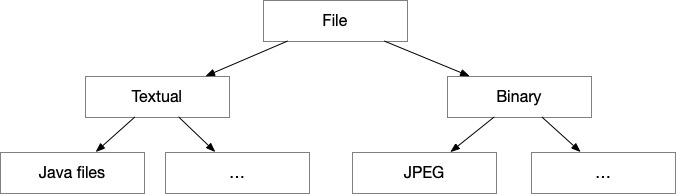
\includegraphics[width=0.5\textwidth]{Taxonomy.jpg}
    \caption{Example of a file type's taxonomy}
    \label{fig:taxonomy}
\end{figure}



We defined a set of metrics as can be seen in \autoref{table:metricsT}. We collect the file's size, the number of Lines of Code (LOC), the number of Source Lines of Code (SLOC) by ignoring comments and empty lines, and the number of lines added and removed. These are basic source code metrics to demonstrate our approach. The list can be extended with additional metrics depending on the purpose.


\section{Visualization}
We represent a ProjectHistory with two kinds of visualization: a 2D visualization, which uses a matrix and works better with small systems, and a 3D visualization. 


\subsection{2D Representation}
This visualization is based on the Evolution Matrix approach by Lanza \cite{Lanza2001}, but adapted to our more flexible evolution model.

A ProjectHistory is a holder of ProjectVersions and FileHistories. 
A ProjectVersion represents a commit, and a FileHistory represents the history of a file. 
The connection between these two entities is a FileVersion that describes the state of a file in a system's version. \\
We can represent a ProjectHistory as a matrix with the following properties: 
\begin{itemize}
    \item Each column of the matrix represents a ProjectVersion, a commit of the repository. 
    \item Each row of the matrix represents a FileHistory, the history of a file. 
    \item Each cell of the matrix represents a FileVersion, the state of a file at a specific point in time defined by the commit. 
\end{itemize}

An empty cell represents a FileHistory (i.e., row) that was not modified in a ProjectVersion (i.e., column). 
This concept was not present in the Evolution Matrix of Lanza because its model worked with SVN, and thus, it worked with incremental snapshots.  

\begin{figure}[h]
    \center
    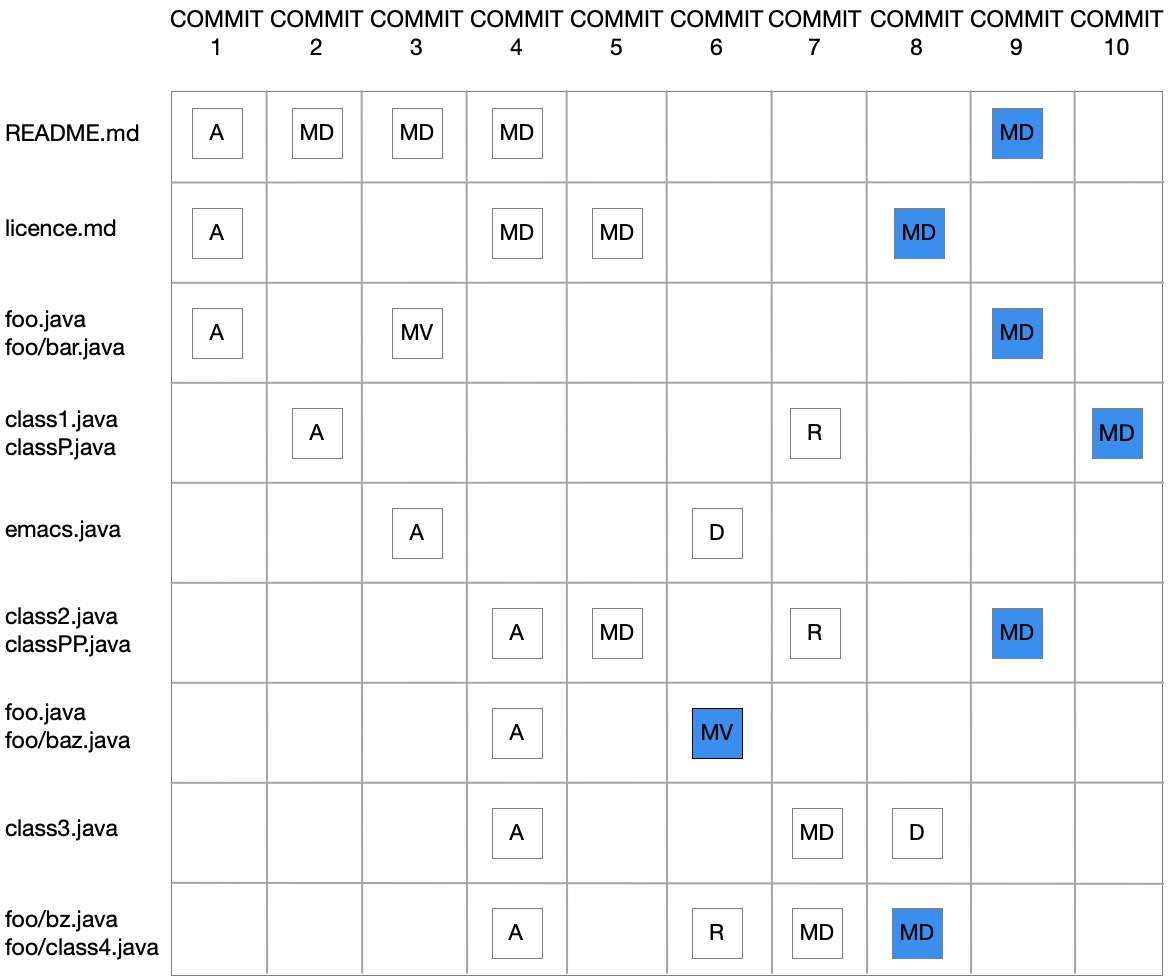
\includegraphics[width=0.6\textwidth]{2DMatrix.jpg}
    \caption{2D Representation of the structural evolution of a repository}
    \label{fig:evolutionMatrixApproach}
\end{figure}
\autoref{fig:evolutionMatrixApproach} depicts the evolution of a repository with 14 files and 10 commits. In this figure we only show the structural evolution of a repository, without considering file metrics as Lanza did. 
Each row represents the history of a file; therefore, it is associated with a set of FileVersions represented by the squares inside each cell. Actions on a file are labeled as: A for ADD, MD for MODIFY, MV for MOVE, R for RENAME, and D for DELETE.
As we can see, the first action made on each file is an ADD. Some files end their history with a DELETE. Notice that \texttt{foo.java} and \texttt{foo/bar.java} are represented by the same FileHistory because they represent the same logical entity in the system. 
In commit $C_3$, \texttt{foo.java} was moved under \texttt{foo/} and renamed to  \texttt{bar.java}.
The same goes for \texttt{foo.java} and \texttt{foo/baz.java} represented by the seventh FileHistory.

We can read this matrix as follows:
 \begin{itemize}
     \item \textbf{Vertically (by rows)}, if we are interested in the history of a particular entity. 
     For example, the FileHistory represented by the first row in \autoref{fig:evolutionMatrixApproach} represents the history of \texttt{README.md}, that was added in the first ProjectVersion (commit $C_1$) and then modified in the second, third, fourth, and ninth ProjectVersion.
     \autoref{fig:evolutionMatrixApproach} is an excellent example of why we cannot rely only on the file name to identify a system's entity. 
     We notice that \texttt{foo.java}, represented by the third FileHistory, was added with the first ProjectVersion and then moved with the third into \texttt{foo/bar.java}. 
     Then, in commit $C_4$, a new file \texttt{foo.java} was added. Nonetheless, the name of the files are the same, they represent two different entities. 
     \item \textbf{Horizontally (by columns)}, if we are interested in which entities were updated on each ProjectVersion. 
    For example, on the first ProjectVersion, we have added the \texttt{README.me} file, the \texttt{licence.md} file, and the \texttt{foo.java} file. 
 \end{itemize}

\autoref{fig:evolutionMatrixApproach} also provides an example of how we reconstruct the system's state after a commit. 
As we have seen, a ProjectVersion does not represent a system snapshot.
Instead, it represents only the changes made to the previous version. 
To reconstruct the system's state at a specific version, we need to consider, for each FileHistory, the last change before that version. 
Under those circumstances, for each FileHistory, we must go back in time until we find the rightmost change. Of course, if the rightmost difference was a DELETE, we ignore the related FileHistory.
In \autoref{fig:evolutionMatrixApproach}, the state of the system after $C_{10}$ is composed of the FileHistories that hold a row with a blue square. 



\subsection{3D Representation}
\label{s:3DRepr}
We aim to make an interactive 3D representation to ease the comprehension task of a developer. Interactive visualizations help users understand more information than a non-interactive version of the same graph. The interaction allows the user to discover a connection among the visualization elements. It is not easy to achieve the same result with a static visualization. For example, if we look at the graph of a repository activity on GitHub\footnote{\url{https://docs.github.com/en/repositories/viewing-activity-and-data-for-your-repository/analyzing-changes-to-a-repositorys-content\#visualizing-additions-and-deletion-to-content-in-a-repository}}, we cannot understand which file was modified at a given time. 

One advantage of our approach is the possibility of having multiple sources of information displayed simultaneously. We aim to make system analysis easier by using human senses and leveraging synesthesia. The phenomenon of synesthesia occurs when stimulation of a sense or a cognitive pathway leads to the involuntary stimulation of another reason or a cognitive path. We experience synesthesia when two or more events are perceived as the same. 
For example, synesthetic people might associate the red color with the letter D or the green color with the letter A. 
There are many forms of synesthesia, each representing different perceptions, such as visual forms, auditory, and tactile.

To visualize a project, we introduce the concept of \textbf{view}. We define a view as a way to illustrate the evolution of a project given a set of specifications. This set of specifications determines how the view must be built. For example, if we want to traverse the repository history by year, this information is part of the specification. A view holds a set of frames, called \textbf{AnimationFrame}, each representing the repository's state at a specific moment. Therefore, the entire history of the repository is displayed by rendering these AnimationFrames sequentially, like in a movie. 

Each repository has a unique history. There are young repositories whose history is one year long and old repositories with more than ten years of development activity. Many repositories are inactive on GitHub, whereas others might have a vast number of contributors raising the total number of commits daily. Therefore, we cannot provide a static approach to traverse the history of a repository. 
Every visualization has its own goal and its way of traversing time. For this reason, we provide two visualization strategies to group commits into AnimationFrames. Both of them traverse the whole history from the beginning until the end.
\begin{itemize}
    \item{Grouping by commits}: the user specifies the number of commits (\texttt{n}) and we create one AnimationFrame for every \texttt{n} commits. With this strategy, the concept of time is lost because we consider only the position of the commit in the commit tree.
    \item{Grouping by timestamp}: the user specifies a time window (\texttt{ts}) and we create one AnimationFrame for every \texttt{ts} seconds. All the commits inside the time window are part of the AnimationFrame. Therefore, we might have empty AnimationFrames if no commits are made in that time window.
\end{itemize}

\autoref{fig:TimeWindowExamples} shows an example of three strategies applied over the same history. In \autoref{fig:TimeWindow1} we made an AnimationFrame every three commits, and as a result, the notion of time is lost. With a commit grouping strategy, we never have an empty AnimationFrame. In \autoref{fig:TimeWindow2} and \autoref{fig:TimeWindow3} the situation is different as they have empty AnimationFrames.
Overall, the examples highlight the importance of a well-designed time window and underline our need to leave the user the choice of the time window's length. For example, younger repositories might have a daily time window, while older repositories might have a weekly, monthly, or yearly view. 

\begin{figure}
    \begin{center}
        \begin{subfigure}{1\textwidth}
            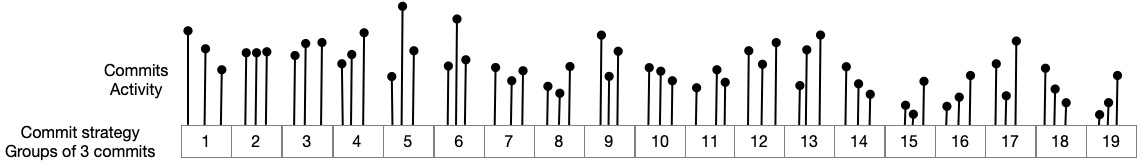
\includegraphics[width=\linewidth]{TimeWindow1.jpg}
            \caption{Grouping every three commits} 
            \label{fig:TimeWindow1}
        \end{subfigure}
        \begin{subfigure}{1\textwidth}
            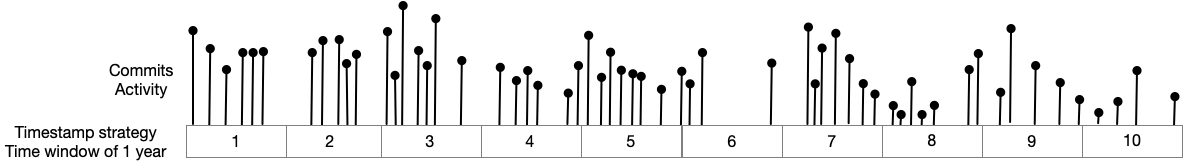
\includegraphics[width=\linewidth]{TimeWindow2.jpg}
            \caption{Grouping every year} 
            \label{fig:TimeWindow2}
        \end{subfigure}
        \begin{subfigure}{1\textwidth}
            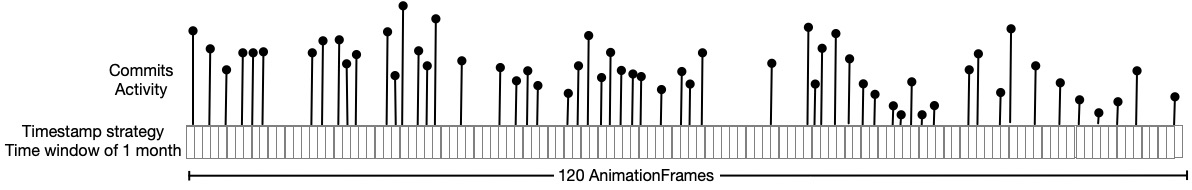
\includegraphics[width=\linewidth]{TimeWindow3.jpg}
            \caption{Grouping every month}
            \label{fig:TimeWindow3}
        \end{subfigure}
        \caption[Example of three different grouping strategies]{Example of three different grouping strategies applied over a system whose history is ten years long with 57 commits}
        \label{fig:TimeWindowExamples}
    \end{center}
\end{figure}



To represent the system's state, an AnimationFrame holds a set of \textbf{ViewFigures}, each representing a file of the system.

A ViewFigure holds a set of properties used by the render process to draw a glyph representing a file. 

\subsubsection*{Layout}
A layout specifies how graphical entities should be laid out. 
Various layout strategies have been proposed to visualize software evolution.
One of the most famous approaches is the city metaphor \cite{Wettel2007}, presented by Wettel \& Lanza, where a file's position depends on its package. It works very well with small and medium systems, and they stated that the interactivity and navigability could be substantially slowed down with large systems.

Our main goals are scalability and incrementality. The visualization needs to scale, even with a very large repository, and it must visualize the system's evolution incrementally. Therefore, the user can immediately distinguish older files from newer ones.

Under those circumstances, we adopted a spiral layout with an outward direction. It is shown in \autoref{fig:layout}. We set a constant gap between entities representing files. 
Older files are positioned at the center of this spiral, whereas newer files are always close to borders. 

We added the \textit{position} property to a ViewFigure to describe its location in the 3D environment. 

\begin{figure}
    \center
    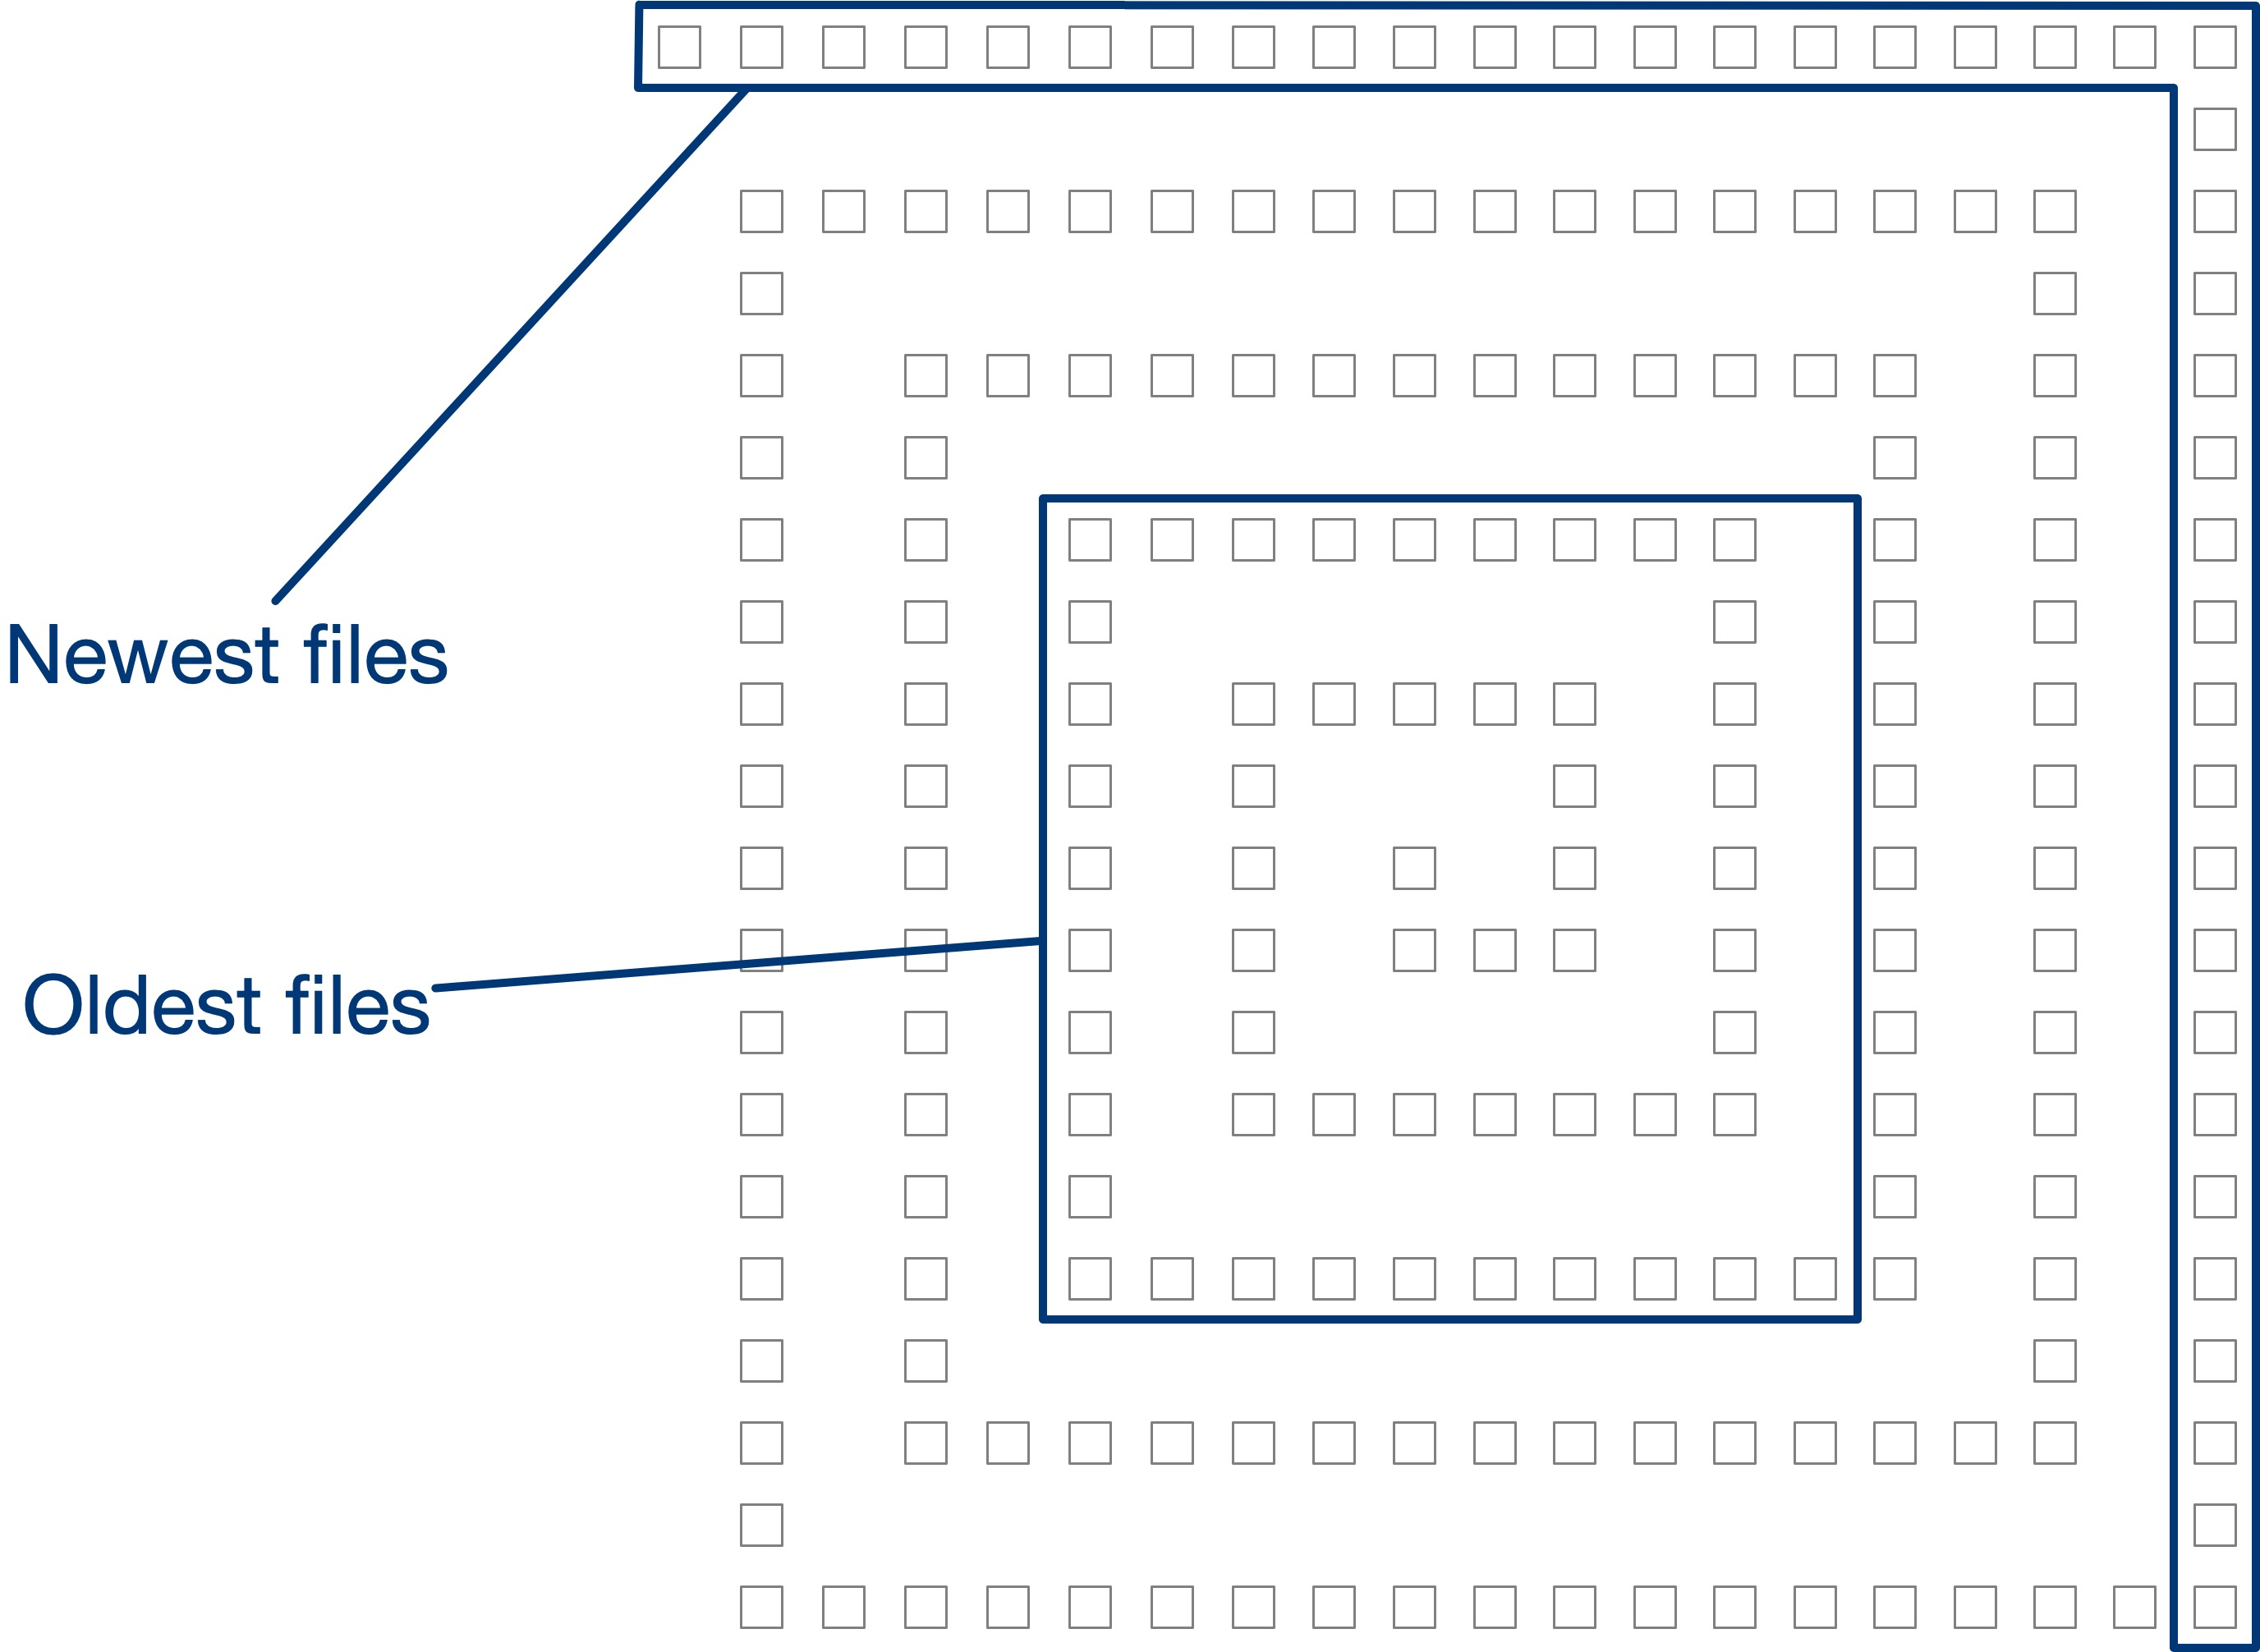
\includegraphics[width=0.7\textwidth]{SpiralLayout.jpg}
    \caption{Outward spiral layout}
    \label{fig:layout}
\end{figure}

\subsubsection*{Color}

Synesthesia occurs when we experience an involuntary stimulation of a cognitive path during the stimulation of another sense.
We present how we use color to describe file actions and simulate how time passes between actions.
As a result, we decided to map each git action with color (see \autoref{fig:ColorAssociation}). This mapping can be personalized through the \textit{color} property of ViewFigure.

In addition to the color, each ViewFigure has another property: \textit{age}. It represents the time elapsed between the last action made on a file and the currently displayed AnimationFrame. 
We selected two strategies to compute the age of an entity:

\begin{itemize}
    \item{Aging by commits}: the user specifies the number of commits (\texttt{n}), and then after \texttt{n} commits, the age of a file is incremented. 
    \item{Aging by timestamp}:  the user specifies a time window (\texttt{ts}) and then after \texttt{ts} seconds the age of a file is incremented.
\end{itemize}

When an action is made on a file, its age is reset to zero. 

The user also can set the maximum age.
When reached, the color of the entity must be equal to the \texttt{base color} chosen by the user.
 
We initially set the base color equal to grey.
\autoref{fig:Aging} provides an example of how the color of an entity changes toward the base color. In this figure, we used green as the base color and represented additions with ten aging steps. 


All the files shared the same criteria to compute the age. The primary purpose of the aging is to immediately distinguish files modified recently from files modified in past AnimationFrames.

\begin{figure}
    \center
    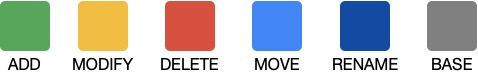
\includegraphics[width=0.5\textwidth]{ColorMapping.jpg}
    \caption{Mapped colors to git actions}
    \label{fig:ColorAssociation}
\end{figure}


\begin{figure}
    \center
    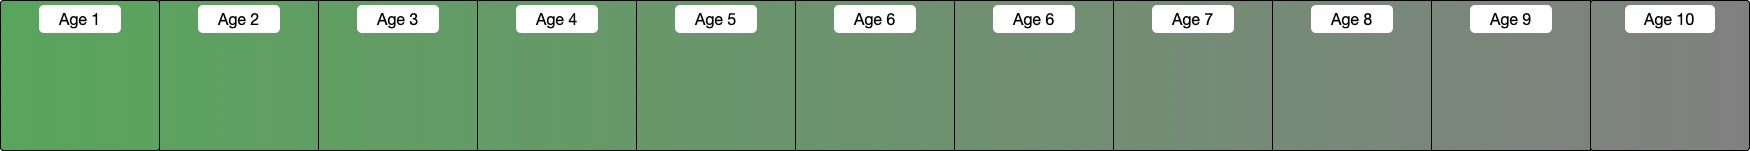
\includegraphics[width=\textwidth]{Aging.jpg}
    \caption{The aging process of an entity whose last action was an ADD and the maximum age is 10}
    \label{fig:Aging}
\end{figure}



\subsubsection*{Shape and Opacity}
To easily distinguish file types, we added a \textit{shape} and an \textit{opacity} property to a ViewFigure.

We did not set a pre-defined set of shapes because we preferred to let each implementation have its own set of models. This was done because it is not guaranteed that all the visualization libraries share the same model. The idea is to map each file type with a shape previously selected by the user. 

Opacity was also added to allow the user to emphasize file types if needed. 


\subsubsection*{Height}
An important piece of information we want to represent is the value of a metric. SYN computes the values of a set of metrics, so we let the user choose his preference to map metrics to the files' height. \\


\autoref{fig:ApproachMapping} summarizes what we said so far. To visualize a Git repository, we use a view, a class that holds all the information needed to render it on screen. To depict the evolution, we traverse the repository's history by a group of commits (generated with a time window or every n commits). Each group is represented by an AnimationFrame, which holds a set of ViewFigures representing a file. The ViewFigure's position is used to describe the creation date of a file. The last action determines the color and age. A chosen metric is used to compute the height of the ViewFigure, and finally, the file type is mapped to shape and opacity. 


\begin{figure}
    \center
    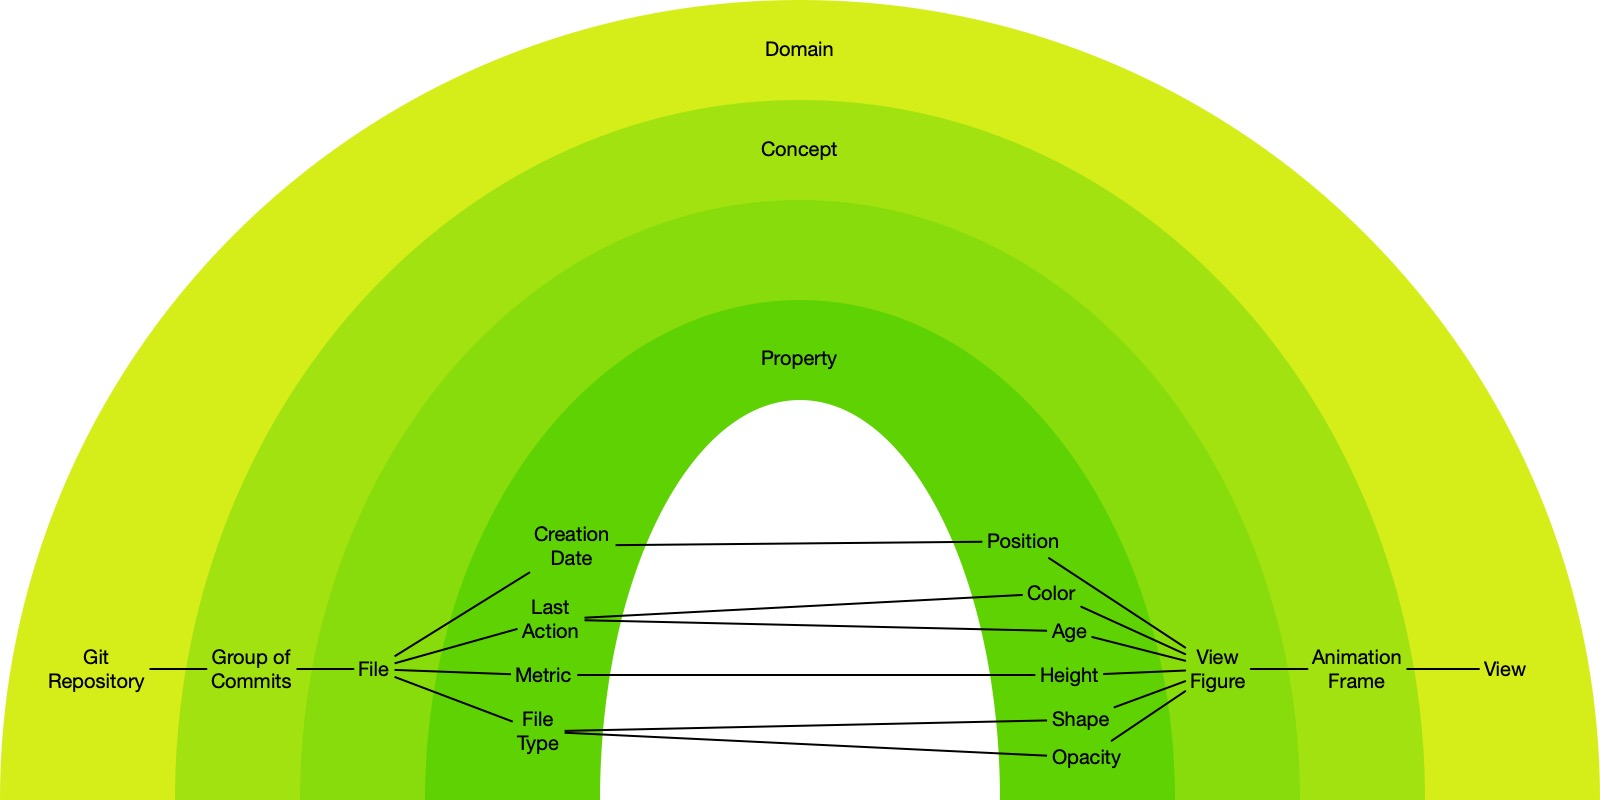
\includegraphics[width=\textwidth]{ApproachMapping.jpg}
    \caption{Mappings of file properties and metrics to view specifications}
    \label{fig:ApproachMapping}
\end{figure}


\newpage
\section{Evolution Auralization}
\label{sec:audioApproach}
In the previous sections, we detailed our approach to visualizing the evolution of a software system. In addition to sight, our approach also stimulates another sense: hearing. To complement our evolutionary visualization, we devised an approach to \emph{\quotes{auralize}} the evolution of a software system. Auralization is a term introduced to be used in analogy with visualization to describe rendering audible (imaginary) sound fields \cite{kleiner1993}. The intuition is to create a melody, starting from the evolutionary data extracted from the version control system, to augment our visualization with complementary pieces of information.


Many parameters influence a musical composition, such as beats per minute (i.e., BPM), pitch, or note. In our approach, we consider the following parameters:

\begin{itemize}
    \item \textbf{Tempo}: indicates the speed of a musical composition. It is measured in BPM. 
    \item \textbf{Measure}: represents a single unit of time featuring a specific number of beats. In our approach, this value is constant (i.e., 1 second). For every measure, we play a new AnimationFrame.
	\item \textbf{Pitch}: is the quality that makes it possible to judge sounds as \quotes{higher} and \quotes{lower} in a sense associated with musical melodies.
	\item \textbf{Amplitude}: determines how loud a note is (i.e., volume).
\end{itemize}

According to Vickerts \cite{Vickers2004}, to distinguish between different activities on the code, we need an \emph{\quotes{orchestral model}} where each instrument represents a certain activity. Following this idea, our approach is composed of three instruments, each representing a different aspect of the evolution of a software system:

\begin{itemize}

    \item \textbf{Bass drums} represents the \textbf{number of commits} in an AnimationFrame. We use this instrument also to dictate the \textbf{Tempo} of our musical composition: the higher the number of commits, the higher the tempo. We normalized the values in the interval $\left[60,200\right]$. The \textbf{amplitude} of this instrument is constant.
    
    \item \textbf{Bass sound} represents the number of \textbf{deleted files} in an AnimationFrame. We use the number of deleted files to determine the repetition and the amplitude of the sound. We divided the measure into quarters and play this instrument one to four times depending on the value of the metric represented. We linearly normalized the amplitude in the range $\left[0.1,0.8\right]$ depending on the metric's value.
    
    \item \textbf{Electric sound} represents the number of \textbf{added files} in an AnimationFrame. We use the number of deleted files to determine the repetition and the amplitude of the sound. We divided the measure into octaves and play this instrument one to eight times depending on the value of the metric represented. We linearly normalized the amplitude in the range $\left[0.2,0.85\right]$ depending on the metric's value.

\end{itemize}

The output of our approach is a musical composition representing a system's evolution. It should be noted that we obtained the parameters mentioned above by tuning the musical composition to our preference However, the approach is customized with different metrics or different thresholds. 


\begin{figure}
    \center
    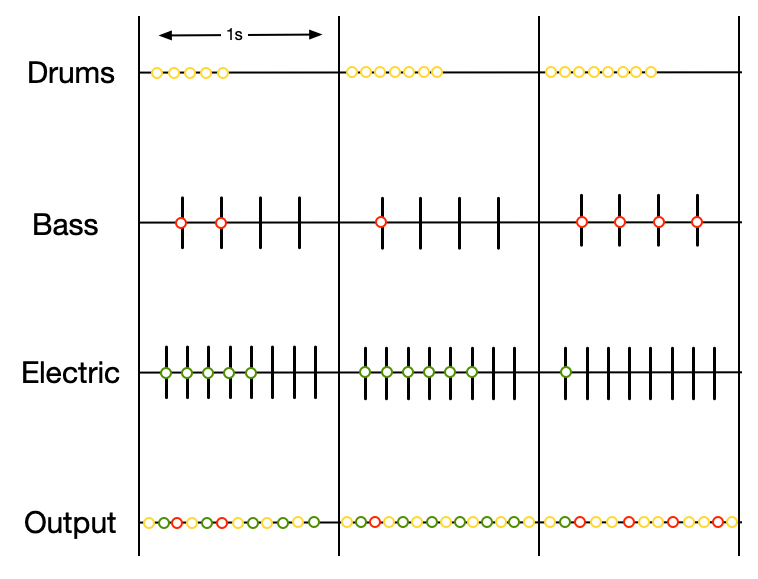
\includegraphics[width=0.5\textwidth]{AuralizationApproach.jpg}
    \caption{Example of how the auralization approach works}
    \label{fig:ApproachArualization}
\end{figure}

\autoref{fig:ApproachArualization} provides an example of how this approach works. Each column represents a measure with a constant value of 1 second. Each row represents one instrument, except for the last, which represents the output composition. The number of notes played from each instrument depends on the value of the respective metric. Therefore, in all the measures was recorded an intense activity, especially in the third one. The number of deleted files was lower in the first two measures than in the last. Consequently, the final output is composed of a few bass notes on the first two measures and four bass notes on the last measure, the most active of this example. The same rules were applied for the electric sound, representing the number of added files.    


\chapter[Implementation]{Implementation}
\graphicspath{ {images/implementation} }
In this chapter, we present how we designed and implemented SYN, a tool that implements the software evolution comprehension approach 
defined in section \ref{s:EvolutionModel} and \ref{s:3DRepr}. 
In section x we provide an overview of our platform by looking at all the modules that compose the architecture. 
In section x we present the user interface of the tool and finally in section x we detail how we implemented the auditory part. 


\section{Platform overview}

SYN is a platform tool that allows developers to have a visual and auditive depiction of an evolving system. 
It was designed to be extensible and efficient, therefore, we created a set of modules each one with its own responsibility:
\begin{itemize}
    \item \textbf{SYN Core}: this is the core module, required by other modules. It holds the core concepts of SYN, such as ProjectHistories, ProjectVersions, and so on. It also provides some abstract concepts that are open to any kind of implementation to achieve the extensibility goal.
    \item \textbf{SYN CLI}: this module is responsible to provide a Command Line Interface to the user.
    \item \textbf{SYN Analyzer}: this module implements the analysis approach described in section \ref{s:EvolutionModel}. 
    \item \textbf{SYN Server}: this module provides some GraphQL endpoints to retrieve data from SYN and display them in a user interface. 
    \item \textbf{SYN Debugger}: this is the user interface of SYN developed to debug and visually depict the information retrieved during the analysis. 
\end{itemize}

All the modules of SYN are written in Java with the exception of SYN Debugger which is written in TypeScript. 

The modular architecture of syn allows the user to interact with the tool in two different ways: through the console with the commands provided by SYN CLI or through a web application embedded inside SYN Debugger. \\
It can be used to explore analysis made on any kind of system since it is language agnostic. Figure \ref{fig:architecture} provides an high-level overview of the architecture. 
The backend enclosed inside SYN Server is written in Java and built using SpringBoot, an open-source framework used to create production-ready microservices.  

...... Explain img modules


\begin{figure}
    \center
    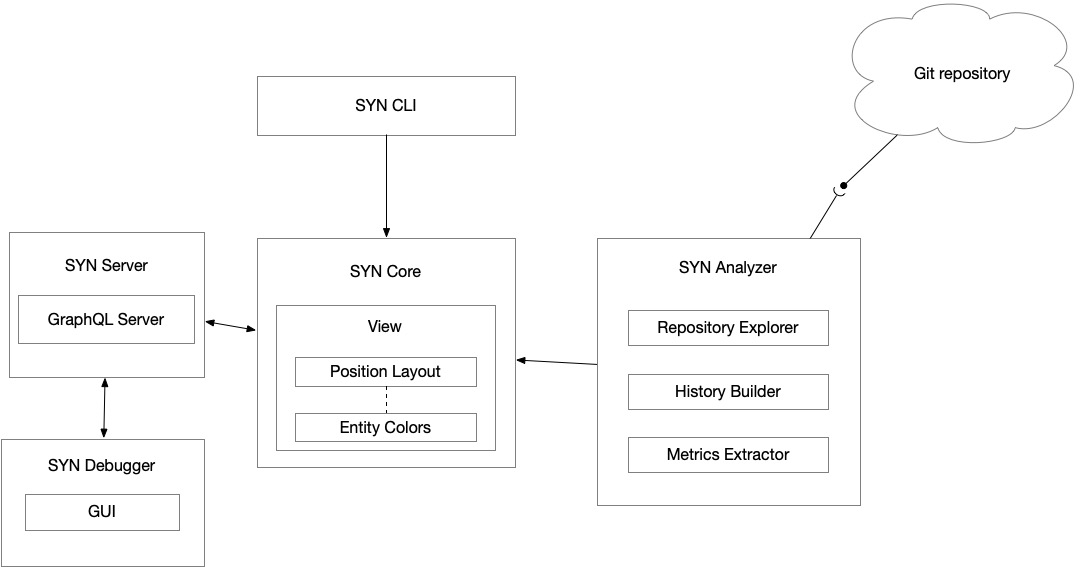
\includegraphics[width=\textwidth]{SYNArchitecture.jpg}
    \caption{Architecture of SYN}
    \label{fig:architecture}
\end{figure}


In our platform, the goal of extensibility is achieved because a developer could easily implement a new analysis approach by developing a new module. 

\section{SYN Core}
SYN Core is a module that holds all the entities that we have introduced in section \ref{s:EvolutionModel}. 
All the classes of our model, extend the \texttt{Entity} class that is composed of the field \texttt{id}, which is unique and is used to identify an object inside our domain. 
To quickly identify the type of the object, each class has an identifier that makes the prefix of the id. 
Classes inside the model of SYN Core could be partitioned into four subdomains: Project, History, Analysis, and View. 

\subsection*{Project}
The fist part of the model consists of the \textbf{Project} entities. 
The diagram is shown in image \ref{fig:modelProject}. The abstract class \texttt{Project} represents a software system. It defines the following fields:
\begin{itemize}
    \item \textbf{name}: the name of the project.
    \item \textbf{projectHistory}: an object that represents the history of the project. It holds the results of the analysis. 
    \item \textbf{path}: the path of the git repository. 
\end{itemize}

Moreover, we defined two additional classes \texttt{LocalProject} and \texttt{RemoteProject} that respectively represent a project that was already cloned and present in the local storage and a project that needs to be retrieved from the internet. 
Therefore, if on one hand, \texttt{LocalProject} does not need any further fields to represent a local project on the other hand \texttt{RemoteProject} needs at least the \texttt{projectURL} field. We might add more information such as the git branch, and the remote credentials but we decided to keep the implementation as simple as possible. 

\texttt{LocalProject}

\begin{figure}
    \center
    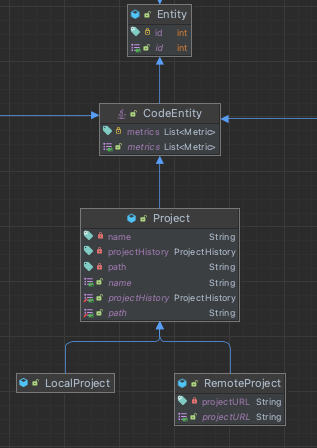
\includegraphics[width=0.2\textwidth]{UMLProject.png}
    \caption{Model: Project entities}
    \label{fig:modelProject}
\end{figure}

\subsection*{History}

\begin{figure}
    \center
    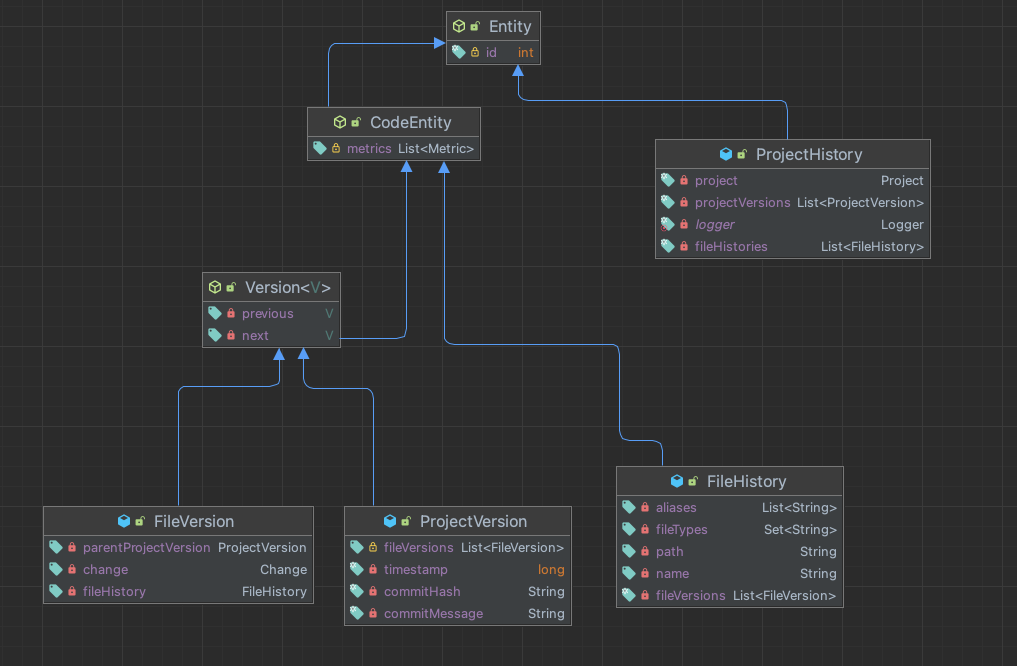
\includegraphics[width=0.2\textwidth]{UMLHistory.png}
    \caption{Model: History entities}
    \label{fig:modelHistory}
\end{figure}

As we evidenced above, each project might hold \textbf{ProjectHistory} object that represents its history. 
Following what we have explained in section \ref{s:EvolutionModel}, the ProctHistory class holds a group of ProjectVersion and a group of FileHistories. The FileHistory class, which represents the history of a single file, consists of:
\begin{itemize}
    \item aliases: a list of paths related to the file. We know that a file is identified by a single unique name. However, since our approach is tolerant to moving and renaming activities, we have to store somewhere all the paths that a file had. In section X we explain the importance of this field and why it has such a crucial role in our analysis. 
    \item fileTypes: A set of Strings each one representing the type of this file. 
    \item Path: the path of the file.
    \item Name: the name of the file.
    \item fileVersions: a list of FileVersions related to this fileHistory. 
\end{itemize}
With the \texttt{VersionV} class we want to represent the state of an entity at a particular point in time. 
The generic parameter \texttt{V} is used as a constraint to force a consistency of the type of the previous and the next version. 
The \texttt{ProjectVersion} class, used to represent git commits, defines the following fields: 
\begin{itemize}
    \item fileVersions: a list of FileVerions that are part of this commit.
    \item timestamp: The timestamp of the commit. 
    \item commitHash: the hash of the commit. 
    \item commitMessage: the message of the commit.
\end{itemize}
Extending the Version class, the ProjectVersion class inherits also the previous and next field that could be used to traverse the history similar to how we traverse a LinkedList. 
Finally, the \texttt{FileVersion} class has the following fields:
\begin{itemize}
    \item parentProjectVersion: the ProjectVersion holding this FileVersion instance. It can be used to retrieve the commit's related information such as the timestamp or the message. 
    \item change: an object that represents the action made on that file. 
    \item fileHistory: the FileHistory that represents the file being modified. 
\end{itemize}

A change represents an action made on a file. In our approach, we have identified five different types of changes, and in our implementation, all of them extend the \texttt{Change} class. It is composed of the field \texttt{linesAdded} and \texttt{linesRemoved} each one representing the number of lines added and removed. 
The goal of our model is to be easily extensible. With that in mind, if in a future implementation we want to extend the variety of metrics specifically collected for each kind of change, we just need to extend the relative class and the polymorphic mechanisms of Java will do the rest. 

\begin{figure}
    \center
    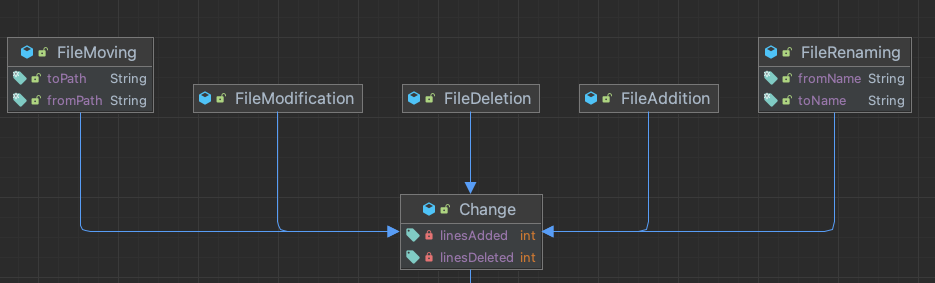
\includegraphics[width=0.5\textwidth]{UMLChanges.png}
    \caption{Model: Change entities}
    \label{fig:modelChange}
\end{figure}


\subsection*{Analysis}
Even though the analysis is effectively implemented into another module, SYN Core provides some abstract classes that need to be implemented to allow the exchange of analysis results. 
The first class that the model defines is \textbf{AnalysisWorkDescriptor}.
An AnalysisWorkDescriptor is, as the name suggests, a holder of useful information to instruct the analyzer on what it has to do. This information comprehends the project on which we have to run the analysis and the list of commits that have to be analyzed. 
The reasons behind this implementation choice are to allow multiple threads to run in parallel multiple analyses without analyzing the same commit multiple times. 
We described this approach in section \ref{s:partialHistoricalRepr}.
\bigbreak

Inside the core module we also have the \textbf{FileTypeManager} class. Its responsibility is to map a set of function to compute evolutionary metrics, (presented in section \ref{s:evolutionaryMetrics}) given a fileHistory. The returned set of functions could be easily extended also with external modules. This choice was made to easily allow external components to increase the set of metrics computed in SYN. In fact, we allow any developer to write any kind of function able to compute any kind of metric and put it inside the set of the corresponding file type. 
We can easily infer the implications of this design, for example, if in the future an engineer wants to write an OO (Object Oriented) metric, such as the number of parents, they can create a function to compute that and associate that function to the "JAVA" or the "OO" type. 
\bigbreak

Finally, in our model, we also defined the \textbf{ProjectAnalysisResult} class. It must be used by an analyzer to return the results that it collected. Moreover, this class made a distinction between partial and total analysis results, allowing it to be used with the partial history retrival approach defined in section \ref{s:partialHistoricalRepr}. The fields declared on this class are:
\begin{itemize}
    \item project: the projects on which the analysis was done.
    \item analysisCompleted: whether if the analysis is partial or total.
    \item timestamp: the timestamp of the moment when the analysis was completed. 
    \item firstCommit: the first commit considered in this analysis. 
    \item lastCommit: the last commit considered in this analysis. 
    \item projectVersions: a list of ProjectVersion discovered during the analysis.
    \item fileHistories: a list of FileHistories discovered during the analysis.
    \item fileVersions: a list of FileVersions discovered during the analysis.
\end{itemize}

Moreover, this module also provides an abstraction of the core concepts of the Git protocol. The classes are \texttt{GitProject}, \texttt{GitCommit} and \texttt{GitChange} each one respectively representing a repository, a commit and a change on a a file. 
With this choice each external module has an high level of autonomy, having the possibility to decide how it should interact with git. 

\subsection*{View}
\label{s:view_impl}
The concept of View in SYN is related to how information should be displayed. In section \ref{s:3DRepr} explained our visual approach. To implement it, we have defined a class called \textbf{View}, that designates how the visualuaziation should be rendered. 
In our visualization approach, we have to display the evolution of a repository. To do that the user interface needs to sequentially display one by one a list of frames, each one representing a moment of the repository. A moment could be either a group of commits in space or a group of commits in time.
We designed the class \textbf{ViewAnimation} to represent a frame of the evolutionary animation of the view. This class has two properties:
\begin{itemize}
    \item \texttt{representedEntities}: a list of ProjectVersions whose data had been used to create that frame.
    \item \texttt{viewFigureList}: a list of ViewFigure each one representing a FileHistory in the view.
\end{itemize}

The \textbf{ViewFigure} class holds graphical properties to properly display each FileHistory
\begin{itemize}
    \item \texttt{position}: the position of the entity.
    \item \texttt{color}: the color of the entity.
    \item \texttt{height}: the height of the entity.
    \item \texttt{shape}: a literal that represents the shape of the entity. 
    \item \texttt{age}: the age of the entity.
    \item \texttt{enabled}: wether the enity should be visualized or not.
    \item \texttt{opacity}: the opacity of the entity.
    \item \texttt{size}: the size of the entity.
\end{itemize}

All these properties are computed when the \texttt{View} object is instantiated. A view is created on the top of the user's preferences. 
So, for example, if the user wants to use a specific color for a specific action, like the dark green for the additions, we have to store this information somewhere. 
This is the reason why we defined the \textbf{ViewSpecification} class. A \texttt{View Specification} is the key element of each view. 
All the views are generated from a \texttt{ViewSpecification} instance. The list of available properties defined inside a \texttt{ViewSpecification} are:
\begin{itemize}
    \item \texttt{versionGroupingStrategy}: the strategy that SYN needs to follow to group up commits and create moments.
    \item \texttt{versionGroupingChunkSize}: the dimension of each group; it can be a number of commits or an amount of time. 
    \item \texttt{colorPalette}: the mapping that SYN has to follow to map FileVersion's actions to colors. 
    \item \texttt{agingGroupingStrategy}: the strategy that SYN needs to follow to define an age.
    \item \texttt{agingStepSize}: the dimension of each age; it can be a number of commits or an amount of time. 
    \item \texttt{agingSteps}: the number of available aging steps. 
    \item \texttt{mapperStrategy}: the strategy that SYN has to follow to compute the height of each entity.
    \item \texttt{mapperStrategyOptions}: optional properties of the mapper if needed.
    \item \texttt{mapperMetricName}: the metric that the mapper should consider to compute the height. 
    \item \texttt{showUnmappedEntities}: wether the view should display entities without the selected metric.
    \item \texttt{fileTypeShape}: the mapping that SYN has to follow to associate a FileType with a shape.
    \item \texttt{fileTypeOpacity}: the mapping that SYN has to follow to associate a FileType with an opacity level.
    \item \texttt{figureSize}: the size of each figure.
    \item \texttt{figureSpacing}: the space between each figure.
    \item \texttt{showDeletedEntities}: wether the view should display deleted eneitites.
    \item \texttt{withGround}: wether the view should include a ground element.
\end{itemize}

Moreover, we defined an abstract class \textbf{PositionLayout} whose implementation specifies how entities should be laid out and a class \textbf{MapperStrategy} whose implementation specifies how the height of the entity is computed. With SYN we ship five possible mapperStrategy:
\begin{itemize}
    \item BucketCountStrategy: where the height of the entity is computed after performing a bucketing on the selected metric's values. 
    \item LinearBucketValueStrategy: where the height of the entity is computed after performing first a bucketing and then a linear mapping on the selected metric's values. 
    \item LinearMapperStrategy: where the height of the entity is computed after performing a linear mapping on the selected metric's values. 
    \item NormalizerMapperStrategy: where the height of the entity is computed after performing a normalization on the selected metric's values. 
\end{itemize}



\section{SYN CLI}
SYN CLI is a command-line interface that allows developers to interact with SYN. It gives to developers full control over the system.
\bigbreak
\textbf{Analysis commands}
\bigbreak

\lstinline{syn analyze auto -p <project_id> -o <output_file> -t <thread_count>}\\
\\
This command is used to run an automatic analysis with SYN. 
Given the id of the project, the system automatically creates all the thread workers (5 by default), runs in parallel the analysis, and joins the results in the output file. 
Moreover, this command ensures that each thread has its own git repository. 
\bigbreak

\lstinline{syn analyze join -o <output_file> <...analysis_file>}\\
\\
This command is used to join analysis results into a single output file.
\bigbreak
\begin{lstlisting}
syn analyze manual -p <project_id> -g <git_repo_path>
    -rc <first_commit> -lc <last_commit> -o <output_file>
\end{lstlisting}
\bigbreak
This command is used to perform a manual analysis with SYN. This command lets the developer have the freedom to choose the repository path and both the first and the last commit of the analysis. 
If the first commit is not specified the analysis starts from the beginning of the history and, in the same way, if the last commit is not specified the analysis ends with the end of the history. 
\bigbreak

\begin{lstlisting}
syn analyze prepare -p <project_id>  -g <git_repo_path> 
    -wn <workers_number> -of <output_folder>
\end{lstlisting}
\bigbreak
This command is used to create a folder of workers to analyze a project.
Based on the number of workers, the repository history is equally partitioned into chunks, and each one is assigned to a worker. 
\bigbreak

\lstinline{syn analyze worker -p <project_id> -g <git_repo_path> -w <worker_file -o <output_file>}\\
\\
This command is used to run the analysis on a project given its worker file. 
Moreover, here the user can specify the git path because it cannot be used by two analyzers at the same time, so it is up to the user to choose a free git repository. 

\bigbreak
\textbf{Prioject commands}
\bigbreak

\lstinline{syn project list}\\
\\
This command is used to print in the console a list of available projects

\bigbreak
\lstinline{syn project create -n <project_name> -p <project_location>}\\
\\
This command is used to create a project given its name and its location. The location could be either a path or an URL. 

\bigbreak
\lstinline{syn project inspect -g <git_path> <project_id> <FileHistory_id>}\\
\\
This command is used to inspect all the FileVersions of a FileHistory. Moreover, if the git repository is provided, SYN performs a double check to ensure that all the FileVersions were spotted. \
To do so, it exploits the output of the command "\lstinline{git log --full-history -- <FileHistory_path>}", keeping attention if the FileHistory's path was changed (git cannot do that).

\bigbreak
\lstinline{syn util csv <project_id> -o <output_file>}\\
\\
This command produces a CSV containing all the commit's tracked information of the selected project. 


\section{SYN Analyzer}
SYN Analyzer is a module that provides an implementation of the analysis approach described in section \ref{s:EvolutionModel}.
To walk through the git-tree, it uses a Java git adapter called JGit. 
To do so, we designed three subclasses of the SYN Core git classes, \texttt{JGitProject}, \texttt{JGitCommit} and \texttt{JGitChange}, that calls the JGit API to retrieve historical information. 
\bigbreak

To run the analysis we need to obtain first an \texttt{AnalysisWorkDescriptor}. 
In this modules, we developed a class \texttt{JGitAnalysisWorkerDescriptorFactory} to partition the commit tree and obtain a set of workers. 
Figure \ref{fig:historysplit} shows an example of a partition with 3 workers. First, the whole history of git is retrieved and stored in memory. Secondly, all the commits from all the branches are merged into a single list sorted by their timestamp. 
Then, the merge commits are removed since the changes recored by them are duplicated and finally the resulting list is partitioned to match the requested number of workers. 
\begin{figure}
    \center
    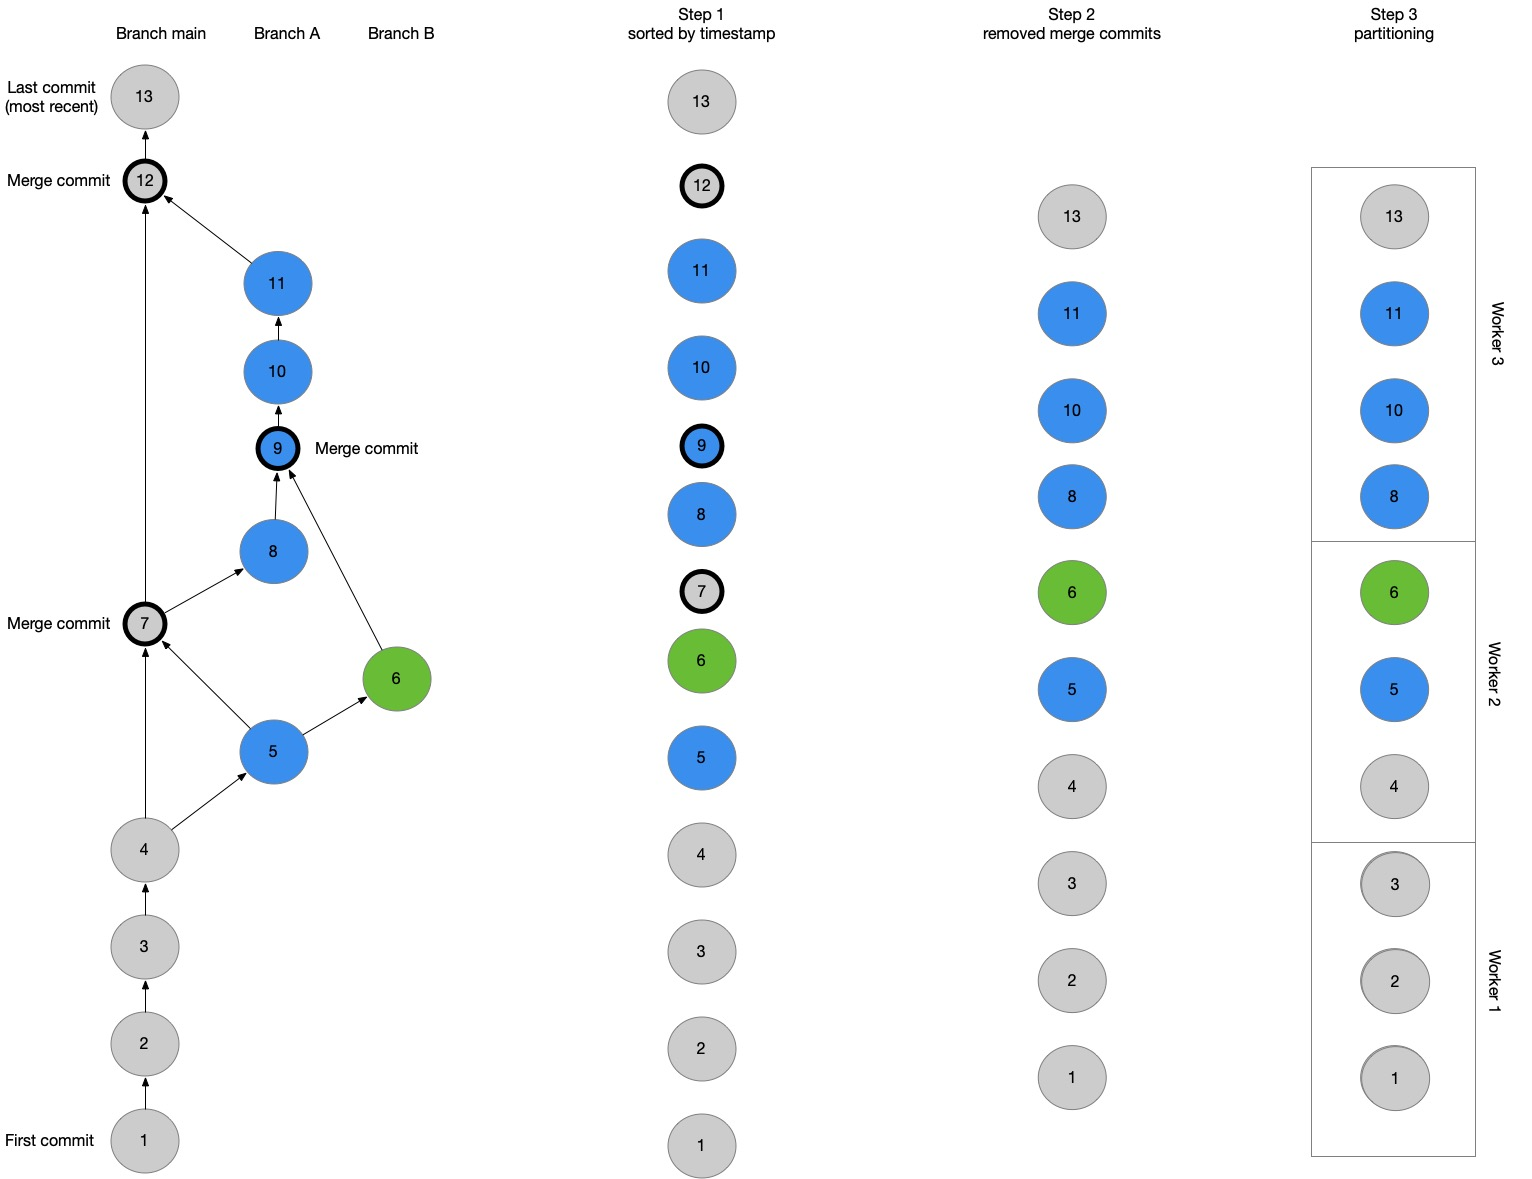
\includegraphics[width=\textwidth]{HistorySplit.jpg}
    \caption{Partition of the commit tree with 3 workers.}
    \label{fig:historysplit}
\end{figure}


The analysis process of a single worker contemplates the following steps:
\begin{enumerate}
    \item we call the method \texttt{runAnalysis} of the class \texttt{ProjectAnalyzer} with a worker descriptor and a project as an argument. 
    \item the analyzer reads the git path of the project and instantates a new \texttt{GitProject}. 
    \item a list of commits, specified in the worker, is retrieved from the \texttt{GitProject}.
    \item the first commit of the list is retrieved, a new \texttt{ProjectVersion} is created with its details. 
    \item the analyzer runs the checkout command of git to restore the version of the system at the one specified by the commit. 
    \item the analyzer retrieves a list of modified files. 
    \item for each modified file, the analyzer creates a new \texttt{FileVersion}, links it with the corresponding  \texttt{ProjectVersion} and \texttt{FileHistory} (creates it if it doesn't not exist yet), and finally extracts all the evolutionary metrics expected for that kind of file.
    \item one all the modified files are analyzed, and the analyzer repeats steps 5, 6, and 7 considering, each time the subsequent commit of the list. 
    \item one all the commits are analyzed, and the analyzer returns all the discovered results within an \texttt{ProjectAnalysisResult} object. 
\end{enumerate}

\bigbreak
If we want to analyze a large repository in an acceptable amount of time, we have to run the analysis in parallel and thus we have to use a considerable amount of workers. 
Each worker produces a \texttt{ProjectAnalysisResult}, then to obtain the full history of the repository we have to all the analysis results. 
In SYN each entity is identified by an id. 
The order in which entities are created is important because we visually sort entities based on their creation timestamp. 
Therefore, having consistency between ids of FileHistory is the most important feature that our algorithm must-have.
We said that each analysis result has: a list of \texttt{FileVersions}, a list of \texttt{ProjectVersions} and a list of \texttt{FileHistories}. 
Analyzers are not able to communicate, therefore each one works in a sandbox. 
When we have to join them, concatenating two lists of \texttt{FileVersions} or two lists of \texttt{ProjectVersions} is not a problem if the historical sequence was respected. 
In fact, these objects are mutually independent of each other.
The challenge comes with \texttt{FileHistories}. When the analyzer encour a file, if it was not discovered yet, it creates a new \texttt{FileHistory} with a new id. 
This sounds like a problem with merging because we might append the same file twice. In other words, we have an issue with linking FileHistories between analysis results.
Assuming for a moment that we do not have this obstacle, there is another situation that might happen, more tricky than the previous one. 
If in the middle of two analysis results a file changed its path, on the first analysis we have an entity with the old path, 
and on the second analysis, we have an entity with a new path. 
Unless we won't keep track of all the possible paths of an entity, it is impossible to reconstruct a connection between these two files. 
This is the reason that brought us to put the alias field in the \texttt{FileHistory} class. 

In the join algorithm that we developed, we employ a map to keep track of FileHistories.
As a result, nevertheless, the file has a different id on any analysis result, the consistency between
FileHistories is guaranteed and moreover, we can guarantee the absence of duplicates inside the newly built repository history. 

Therefore, the algorithm takes as input a list of already discovered FileHistories and an \texttt{ProjectAnalysisResult} and it returns a dictionary.
This dictionary is used to map partialFileHistories, the FileHistory of an analysis result, to definitiveFileHistories, which are part of the full history of the repository. 
To obtain this map it uses the following strategy:
\begin{enumerate}
    \item If the last alias of a definitiveFileHistories is equal to the first alias of a partialFileHistory then they represent the same file.
    \item If in the partialAnalysisResult there is more than one FileHistory with the same first alias, only the first is mapped to a definitiveFileHistories and the other partialAnalysisResult are mapped to a new newFileHistory.
    \item If a partialFileHistory has not an alias match with a previously created definitiveFileHistories then it represents a new definitiveFileHistories.
\end{enumerate}

% \begin{algorithm}
%     \caption{Algorithm to create a mapping between partialFileHistories and definitiveFileHistories}
%     \label{alg:cap}
%     \begin{algorithmic}[1]
        
%     \State $partialToDefinitiveMap \gets new Map()$
%     \State $partialAliasToFileHistory \gets new Map()$
%     \State $newFileHistories \gets new List()$
%     \end{algorithmic}
% \end{algorithm}

\begin{algorithm}
    \caption{Algorithm to create a mapping between partialFileHistories and definitiveFileHistories}\label{euclid}
    \begin{algorithmic}[1]
    \Procedure{PartialToDefinitiveFH}{$projectAnalysisResult, partialFileHistories$}
        \State $partialToDefinitive \gets Map()$
        \State $partialAliasToFH \gets Map()$ \Comment{Strategy 1}
        \State $unmappedPartialFileHistories \gets List()$  \Comment{Strategy 2}
        \ForAll{partialFH in partialFileHistories}
            \State $firstAlias \gets partialFH.aliases[0]$
            \If{$!partialAliasToFH.has(firstAlias)$}
                \State $partialAliasToFH.set(firstAlias, partialFH)$  \Comment{Strategy 1}
            \Else
                \State $unmappedPartialFH.append(partialAliasToFH)$  \Comment{Strategy 2}
            \EndIf
        \EndFor

        \ForAll{definitiveFH in projectAnalysisResult} \Comment{Strategy 1}
            \State $lastAlias \gets definitiveFH.aliases[definitiveFH.length - 1]$
            \If{$partialAliasToFH.has(lastAlias)$}
                \State $partialFH = partialAliasToFH.get(lastAlias)$
                \State $definitiveFH.path = partialFH.path$
                \State $definitiveFH.aliases.addAll(partialFH.aliases)$
                \State $partialToDefinitive.set(partialFH, definitiveFH)$
                \State $partialAliasToFH.remove(lastAlias)$
            \EndIf
        \EndFor

        \State $unmappedPartialFH.addAll(partialAliasToFH)$ \Comment{Strategy 3}
        \ForAll{partialFH in unmappedPartialFH} 
            \State $definitiveFH = FileHistory(partial.name, partial.path)$
            \State $definitiveFH.aliases = partialFH.aliases $
            \State $partialToDefinitive.set(partialFH, definitiveFH)$
        \EndFor
        \State \textbf{return} $partialToDefinitive$
    \EndProcedure
    \end{algorithmic}
\end{algorithm}


\section{SYN Server}
SYN Server is responsible for providing the elaborated information, given by the analysis results, in an intermediate language between the 
front-end (SYN Debugger) and the back-end. We used SpringBoot, a Spring-based tool for developing "production-ready" applications efficiently.

\subsection*{GraphQL API} 
This type of communication is used in SYN for retrieving repository information.
GraphQL is a query language for APIs that gives clients the possibility to ask for exactly what they need.
This is an advantage compared to a REST API because, instead of always returning a predefined set of data, with GraphQL only the needed information will be returned making the communication more effective. 
In GraphQL endpoints are divided into queries and mutations. Queries are used to retrieve data while mutations are used to create or alter data. 

\bigbreak
\textbf{Mutations}

=> \texttt{createProject(projectName: String!, projectLocation: String!): Project} 
used to create and automatically analyze a new project.
It takes as parameters the name of the project and its location (the path on the local machine or the URL), both as a String. 

\bigbreak
\textbf{Queries}

\texttt{projectList:  [PartialProjectInformation]!} \\ 
is used to retrieve a list of projects. For performance reasons, with this query only the name and the id of a project can be retrieved. 
\bigbreak
\texttt{view(projectId: Int!, viewSpecification: ViewSpecificationInput!): View} \\
returns a view of the project identified by the argument \texttt{projectId}, built following the directives specified in the \texttt{viewSpecification} object. 
This query returns an object representing a view, thus it has all the fields that we have described in section \ref{s:view_impl}. 
\bigbreak
\texttt{partialView(projectId: Int!, viewSpecification: ViewSpecificationInput!, viewAnimationId: Int): View} \\
returns a view with only the next 100 animations starting from the one identified by \texttt{viewAnimationId}. 
This endpoint was created to enable performance optimizations on clients. If the viewSpecification expected too many animations, the resulting view would be a bottleneck for the client.
With this endpoint it can still retrieve the view, and then animation can be lazily loaded once they are effectively required. 
\bigbreak
\texttt{fileHistory(projectId: Int!, fileHistoryId: Int!): FileHistory} \\
used to retrieve details of the FileHistory identified with \texttt{fileHistoryId} of the project identified with \texttt{projectId}.
\bigbreak
\texttt{projectVersions(projectId: Int!, projectVersionsId: [Int]!): [ProjectVersion]!} \\
used to retrieve details of the ProjectVersion identified with \texttt{projectVersionsId} of the project identified with \texttt{projectId}.
\bigbreak
\texttt{groupingPreview(projectId: Int!, viewSpecification: ViewSpecificationInput!): Int} \\
this endpoint is used to compute the number of AnimationFrames that are gonna be created with the given \texttt{viewSpecification}.
\bigbreak
\texttt{fileTypeCounter(projectId: Int!): [FileTypeCounter!]!} \\
this endpoint returns a list that maps each FileType with the number of occurrences that it has in the project \texttt{projectId}.
\bigbreak
\texttt{fileTypeMetrics(projectId: Int!, fileTypeFilter: [String]): [FileTypeMetrics!]!} \\
this endpoint returns a list that maps each FileType with a list of metrics available for it. Only the FileTypes specified in the \texttt{fileTypeFilter} list are considered. 


\section{SYN Debugger}

SYN Debugger is a web application that allows developers to interact with SYN. It is written with React.js, a popular JavaScript framework. 
The aim of this application is to have a visual depiction of the view generated by the server, plus some additional information. 
For example, it allows you to ckick on an entity and sees the information that is related to it. 
The visualization is based on Babylon.js, a popular 3D library. 
SYN Debugger provides a different kind of customizations to the view, such as the shape and the colors of the entities. 
All these customizations are sent to the back-end server, through a \it{view specification} file. 

The main purpose of this application is to debug the view and explore all the possible visualization combinations of a system. 

\section{SYN Sonic}

....

% \appendix %optional, use only if you have an appendix

% \chapter{Some retarded material}
% \section{It's over\dots}
% \lipsum 

\backmatter


%\bibliographystyle{alpha}
%\bibliographystyle{dcu}

\bibliographystyle{plainnat}
\bibliography{biblio}

%\cleardoublepage
%\theindex %optional, use only if you have an index, must use
	  %\makeindex in the preamble

\end{document}
